\chapter{Quasiparticle Interference (QPI)}
%todo: to write the abstract of this chapter after finishing this chapter
%todo: to standardize the vector form in this chapter 
\section{Introduction to Quasiparticle}
A Quasiparticle is any long-lived, well-defined excitation in a system that behaves like a particle; it is a semi-classical term used to describe particle interactions in terms of renormalized single-particle excitation. In Fermionic systems, it corresponds to a sharp peak in the spectral function: 
	\[
	A(\mathbf{k}, \omega) = -\frac{1}{\pi} \frac{\operatorname{Im} \Sigma(\mathbf{k}, \omega)}{(\omega - \tilde{E}_{\mathbf{k}})^2 + [\operatorname{Im} \Sigma(\mathbf{k}, \omega)]^2},
	\]

This section aims to introduce the concept of a quasiparticle, first through a historical overview of the development of quasiparticle theory, relevant languages and terms will be established, as well as the assumptions and limitations of the theory; then we illustrate the concept quantitatively through a microscopic theory of landau quasiparticles. 

\subsection{The historical overview}
The development of a quasiparticle model for Fermionic systems started in 1940s, when Sommerfeld and Bethe\cite{SommerfeldBethe1933} developed a model for a non-interacting electron gas, also known as the "Fermi gas", in which a series of important terms are introduced. Consider a system made of non-interacting electrons with momentum $k$ and spin $\sigma = 1/2$, which is in touch with an electron reservoir with chemical potential $\mu$. The occupation number follows the Fermi-Dirac distribution $n_{k,\sigma}=1/(1+e^{(k^2/(2m)-\mu)/T}))$. At $T=0$, the occupation thus has a sharp boundary known as the Fermi surface, in the momentum space confined by the Fermi wave number $k_f$, and the energy defined by the Fermi surface is called the Fermi energy. At non-zero temperature, electrons at the Fermi energy will start to be excited above the Fermi energy; this excitation can also be described in second-quantization by the creation of a quasiparticle with energy: $\epsilon_{k,sigma} = k^2/2m - \mu$. 

Sommerfeld's theory of the electron gas worked quite well in standard metallic systems, but the success was unexpected, as the model neglected the Coulomb interaction between electrons. In a metallic system where the electron separation is in the order of the lattice spacing, the Coulomb interaction is in the order of eV, which is much larger than other energy scales, say, the thermal excitation considered in the electron gas mode. 

In the late 1960s, Landau raised a theory of the Fermi liquid with a series of foundational papers\cite{Landau1956,Landau1957} to address that even in the presence of interactions, we can find fermionic excitations in these many-body systems, and describe these excitations with what is known as the Landau quasiparticles. By adding a time-variant interaction term, defined by time constant $\zeta$ to the non-interacting system, and constructing the system Hamiltonian as
\begin{equation}\label{adiabatic}
	H_{\zeta} = H_0 + H_{\text{int}} e^{-\zeta t}, \quad t > 0,
\end{equation}

By the principle of adiabatic continuity, Landau is able to bridge between the states of interacting and non-interacting systems. Consequently, the states describing the interacting system can now be reduced to states in the non-interacting system with the same quantum numbers $k, \sigma$. More specifically, as quoted from \textit{What is a Quasi-Particle?} by J.R.Schrieffer, "these many-body states are well characterized in terms of a set of elementary excitations, called quasi-particles, which for the interacting system plays the same role as the excited electrons (above the Fermi surface) and the excited holes (below the Fermi surface) in the Independent-particle approximation (IPA)." \cite{schriefferWhatQuasiparticle1970}

Landau's quasiparticle is an extremely useful concept in computing the screening and the transport properties of an electron-gas-like system. However, we should emphasize that the theory is only valid with several assumptions:

For an adiabatic procedure to hold, time scale $\zeta$ in Equation \ref{adiabatic} should be bounded by two conditions: 1. rate of evolution should be small compared to the energy of the state: $\zeta << \epsilon_{k,\sigma}$, 2. the final bound state remains the same as the initial one, meaning the lifetime $\tau_{QP}$ of the bound state should be long enough: $\tau_{QP} >> \zeta^{-1}$. Therefore, $\zeta$ should suits: 
\begin{equation}
	\tau_{QP}^{-1} << \zeta << \epsilon_{k,\sigma},
\end{equation}
since typical excited energy is in the order of temperature, and the lifetime is inversely proportional to $T^2$, we can also write:
\begin{equation}
	T^2 << \zeta << k_B T,
\end{equation}
This requirement can be satisfied at a range of low temperature. Later we will also see that the requirements also extend to the energy level of the states, since the quasiparticle lifetime decreases as energies deviate from the Fermi energy. 
%todo: can refer to the chapter where we talk about the lifetime decay with simulation. 
%Therefore, Landau's theory of Fermi liquid postulated that an interacting fermionic system can we mapped adiabatically to a non-interacting Fermi gas, with long-lived quasiparticle that shares the same quantum numbers near the Fermi surface. 
In electronic systems, the theory works in a regime with weak to moderate electron-electron correlations at sufficiently low temperatures, and thus, it succeeds in explaining the properties of simple and noble metals. For more detailed reading regarding the theory, the textbooks of Pines and Nozieres~\cite{nozieresTheoryQuantumLiquids2018} and Nozieres \cite{nozieresDerivationLandauTheory1962} offer derivations and in-depth discussions. 

Landau’s Fermi-liquid theory, though limited in scope, provided the conceptual foundation for the quasiparticle picture and inspired its formalization within the Green’s function framework of many-body theory. The first step beyond a simple free-electron description came with the Hartree–Fock approximation (1930s), which introduced a self-consistent mean-field treatment of electron–electron interactions and laid the groundwork for systematic diagrammatic expansions~\cite{fockNaeherungsmethodeZurLoesung1930,slaterNoteHartreesMethod1930}. In the 1950s, the Random Phase Approximation (RPA) extended this picture to include dynamical screening, successfully describing collective modes such as plasmons and the optical properties of metals and semiconductors~\cite{bohmCollectiveDescriptionElectron1951,nozieresCorrelationEnergyFree1958}.

A major milestone arrived in 1957 with BCS theory, which provided a microscopic understanding of superconductivity. Near the critical temperature T\textsubscript{c}, Landau quasiparticles become unstable under a weak attractive interaction and form Cooper pairs, spontaneously breaking gauge symmetry. In the superconducting state, the elementary excitations are Bogoliubov quasiparticles, whose finite excitation energy and coherence factors render them well-defined and long-lived in clean superconductors~\cite{cooperBoundElectronPairs1956,bardeenTheorySuperconductivity1957,tinkhamIntroductionSuperconductivity2004}.

Later developments extended the quasiparticle concept to systems with progressively stronger correlations. The GW approximation (1965) improved upon RPA by providing a more accurate treatment of dynamical screening~\cite{hedinNewMethodCalculating1965,aryasetiawanGWMethod1998}. In the 1990s, Dynamical Mean-Field Theory (DMFT) offered a non-perturbative framework to handle strong local interactions, showing that while quasiparticles remain well-defined in moderately correlated systems, they disappear near a Mott transition~\cite{metznerCorrelatedLatticeFermions1989,georgesDynamicalMeanfieldTheory1996}. More recently, the combined GW+DMFT framework has merged non-local dynamical screening with exact local correlations, enabling realistic modeling of heavy-fermion materials and other strongly correlated systems~\cite{biermannFirstprinciplesApproachElectronic2003}. These theoretical advances, while not exhaustive, highlight that the quasiparticle concept remains an approximation whose validity is system-dependent and continues to evolve. A detailed historical overview, including modern applications to topological materials, is given by Wölfle and Abrahams~\cite{wolfleQuasiparticlesCondensedMatter2018}.

\subsection{Microscopic Theory of Quasiparticles}
Landau quasiparticles are added to a system with the creation of excitations, therefore, we need to look at the retarted Green's function $G^R$ as it measures the density of states for adding particles, and thus a system's response to creating or annihilating a single fermion at a given state. We consider the one-particle retarded Green's function: 
\begin{equation}\label{retardedgreen}
	G^R_{k \sigma, \omega} = \frac{1}{\omega -\epsilon_k - \Sigma^R(k \sigma, \omega)},
\end{equation}
where $\epsilon_k= \frac{k^2}{2m-\mu}$ is the free electron energy with respect to the chemical potential $\mu$, and $\Sigma^R_{k \sigma, \omega}$ is the retarded self-energy that is irreducible in diagrammatic expansion. 

We then expand the self-energy into real and imaginary parts, the effective single-electron energy is $\epsilon'_{k} = \epsilon_k + \operatorname{Re}\Sigma^R(k,\omega)$. We can then define the renormalized Fermi momentum $k^*_{F}$ as $\epsilon'_{\tilde{k_{F}}} = 0$. Then we expand $G^R_{k, \omega}$ around $k = k^*_{F}$ and get: 

\begin{equation}
\label{gr_full}
G^{R}(\mathbf{k}, \omega) \approx Z \left[ \omega - \epsilon^*_{\mathbf{k}} + i \Gamma_{\mathbf{k}} \right]^{-1}
\end{equation}
where
\begin{align} 
	Z^{-1} &= 1 - \left. \frac{\partial}{\partial \omega} \, \mathrm{Re} \, \Sigma (k^*_{F}, \omega) \right|_{\omega = 0}, 
	\\ 
	\label{eq2}
	\epsilon^*_{\mathbf{k}} &= (k - k^*_{F}) Z \left. \frac{\partial}{\partial k} \left( \epsilon_{\mathbf{k}} + \mathrm{Re} \, \Sigma ({k}, 0) \right) \right|_{k = k^*_{F}}, \\ 
	\label{gamma}
	\Gamma_{\mathbf{k}} &= Z \mathrm{Im} \Sigma^{R}({k}, 0) 
\end{align}

\noindent here, $\epsilon^*_{\mathbf{k}}$ is the renoramlized energy, $\Gamma_{\mathbf{k}}$ is the relaxation rate which is inverse proportional to the quasiparticle lifetime $\tau_{QP}$, and $Z$ is called the weight factor of qausiparticles. We can further parameterize the renormalized energy with the effective mass $m^*$: 
\begin{equation}\label{energy}
	\epsilon^*_{\mathbf{k}} = \frac{k^*_F(k-k^*_F)}{m^*}
\end{equation}
We can then plug Equation \ref{energy} into Equation \ref{eq2} and get: 

\begin{equation}
	\frac{m}{m^*} = Z(1 + \frac{m}{k^*_F}\frac{\partial}{\partial k}\operatorname{Re}\Sigma(k,0)|_{k = k^*_{F}})
\end{equation}

We can see that by introducing the retarded self-energy that encodes the interaction effects on single particles, we can describe the system near the modified Fermi momentum with quasiparticles. These quasiparticles are characterized by an effective mass $m^*$ that is dictated by the real part of self-energy and a lifetime $\tau_{QP}$ that is inversely proportional to the imaginary part of self-energy. Providing the imaginary part of self-energy is very small, we have long lived quasiparticles, and hence we can write the Spectral function from Equation \ref{gr_full}:
\begin{equation}
	\label{eq.akw}
	A(\textbf{k},\omega) = -2\operatorname{Im}G^R(\textbf{k}, \omega) 
	\approx 2\pi Z\delta(\omega-\epsilon^*_\textbf{k}) 
\end{equation}

This indicate a sharp peak at $\omega=\epsilon^*_\textbf{k}$, thus resembles the spectral function of a Fermi gas, and the pole is what we call the quasiparticle in the Fermi liquid theory. However, we can see that Equation \ref{eq.akw} does not fulfill the normalization rule: 
\begin{equation}
	\int_{-\infty}^{+\infty} \frac{d\omega}{2\pi} A(\textbf{k},\omega) = 1, 
\end{equation}

we need to incorporate another term $A'(\textbf{k},\omega)$ into $ A(\textbf{k},\omega)$ to that has an integrated wight given by 1-Z, giving us: 
\begin{equation}
	\label{eq.akw}
	A(\textbf{k},\omega) = 2\pi Z\delta(\omega-\epsilon^*_\textbf{k}) + A'(\textbf{k},\omega)
\end{equation}
Fig. \ref{fig:ch5_spect} \cite{bruusManyBodyQuantum2004} illustrates this effect, and that term $A'(\textbf{k},\omega)$ captures the remaining excitations other than the well defined quasiparticle pole. 

\begin{figure}
	\centering
	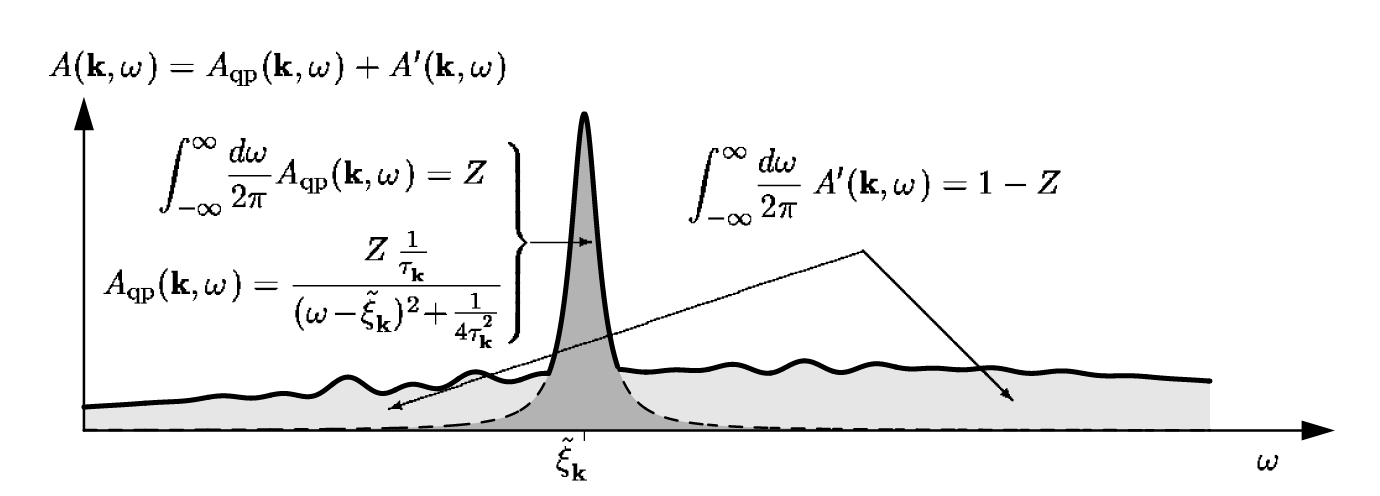
\includegraphics[width=\textwidth]{Ch5_spectralfunciton.png}
	\caption[\textbf{Spectral function $A(\textbf{k},\omega)$}]{\textbf{Spectral function $A(\textbf{k},\omega)$}. The spectral function $A(\textbf{k},\omega)$ that includes the quasiparticle peak and the background function $A'(\textbf{k},\omega)$ stemming from other types of excitation}
	\label{fig:ch5_spect}
\end{figure}

\section{Introduction to Quasiparticle Interference}

In the Fermi liquid theory, an interacting many-particle system is modeled by a renormalized single-particle system, with quasiparticles capturing the excitations near the renormalized Fermi level. These quasiparticles are long-living and carry the same quantum numbers $(\textbf{k}, \sigma)$ as the bare particles. The non-infinite lifetime corresponds to the weakly interacting nature of the quasiparticles; interactions involved quasiparticles include quasiparticles-quasiparticle interaction of the same kind, e.g. the phonon-phonon interaction in anharmonic lattices \cite{kimExploringAnharmonicLattice2023}; quasiparticles of a different kind, e.g. the exciton-phonon coupling in ZnO \cite{mendelsbergPhotoluminescenceExcitonphononCoupling2011}. 

One can utilize the interactions that involve quasiparticles as a channel to explore properties of matters. In particular, when it comes to single-particle properties, or more specifically, probing the spectral function $A(\textbf{k},\omega)$, the tunneling experiment is at a unique position because of its ability to both inject and remove an electron into and out of a many-body system.  

As \ac{STM} combines the ability to resolve both the spatial and energy dimensions of the electron density of states, we can perform a powerful measurement call Quasiparticle Interference measurement, or \ac{QPI} measurement. This section aims to introduce \ac{QPI} measurement, exploring both its theoretical foundation as well as the experimental details. We will then point out challenges of performing and interpreting a "good" \ac{QPI} measurement. This will give a direct motivation for our next chapter, which introduces a method that we use to mitigate some of the challenges. 

\subsection{Terminology}
To set stage for the discussion in this chapter, we must make distinctions between the following terminologies: 
\begin{itemize}
	\item QPI: The interference between the incoming quasiparticle and the outgoing quasiparticle in a scattering event between quasiparticles and lattice imperfections.  
	\item QPI pattern: an interference pattern that can be observed by \ac{STM} on the surface of the material.
	\item QPI measurement: a measurement that measures the QPI patterns presented in systems that intrinsically host QPI. This hints at an assumption that the tunneling experiment did not induce the scattering, but act as a mere observer of this phenomenon.
\end{itemize}
%We should note that STM is not the only tool that can perform QPI measurement. In fact, interference of quasiparticles are reported across a wide literature in different systems using different techniques. For example,
%todo: to wirte different examples here, template as X used Y technique to detect G quasiparticle Interference pattern in Z system.: ranging from crystalline excitation like phonon in Si phononic crystals \cite{maldovan_phonon_2015}, electronic excitation like Bogoliubov quasiparticle in superconductors interference strongly\cite{homan_search_nodate}
I will then elaborate what these terms mean in the context of an STM study, and to reduce redundancy, in the following writing, QPI, QPI pattern and QPI measurement will be referred specifically to STM studies.

\subsection{QPI measurement in STM}
%todo: to plot a standard grid and its FFT here.
Understanding QPI patterns is the first step to understand QPI measurement. A QPI pattern is the modulation of \ac{LDOS} due to quasiparticle-impurity scattering. The modulated \ac{LDOS} provides direct insight on the quasiparticle band structure. Imagine an ideal metal with no crystal imperfection; we know that the Landau quasiparticle has an eigenstate in real space described by a Bloch wavefunction: 

\begin{equation}
\psi(\mathbf{r}) = e^{i \mathbf{k} \cdot \mathbf{r}} u(\mathbf{r})
\label{eq:bloch}
\end{equation} 
where $k$ is the crystal momentum of the quasiparticle. And the electron \ac{LDOS} can be written as  
\begin{equation}
\text{LDOS}(E, \vec{r}) \propto \sum_k |\Psi_k(\vec{r})|^2 \delta(E - \varepsilon(k))
\label{eq:ldos}
\end{equation}

where  $\epsilon(k)$ is the renormalized energy dispersion of the Bloch state for different $\vec{k}$; Remark: from now on all the renormalized energy will be write directly as $\epsilon(k)$ unless otherwise mentioned. And if we plug Equation \ref{eq:bloch} into Equation \ref{eq:ldos}, we see that the $\text{LDOS}$ is translationally invariant at all Bravais-lattice-equivalent points. Thus why in ideal case, real space imaging technique like \ac{STM}, can not be used to measure $\epsilon(k)$. 

However, crystal imperfections can help us introduce a momentum texture to the $\text{LDOS}(E, \vec{r})$. In low temperature STM, where the phonon modes and other excitations are rare or absent, lattice imperfections such as point defects can cause elastic scattering which mix electronic eigenstates at different $\vec{k}$ but at the same energy. The interference between the incoming and outgoing wave forms a "standing wave" that acts as a real space modulation in $\text{LDOS}(E)$. At the Fermi energy, this pattern is described as a Friedel oscillation\cite{benaFriedelOscillationsDecoding2016}. This spatial modulation in $\text{LDOS}$ is the QPI pattern that we refer to in \ac{STM} studies. We can perform \ac{STS} measurement on the region that presents this QPI pattern, then apply a Fourier transform to the STS, allowing us to view this QPI pattern in the momentum space; the q-space QPI pattern is directly related to the quasiparticle band strucutre. This whole process of detecting QPI pattern and analyze it in momentum space is what we call a QPI measurement. 

We will quantitatively showcase this \ac{LDOS} modulation with a simulation on a toy model in the following section. 

%\begin{figure}
%	\centering
%	\includegraphics[width=0.5\textwidth]{example-image-a} % Replace with your image file
%	\caption{Friedel oscillation and QPI}
%	\label{fig:example}
%\end{figure}

\subsection{LDOS modulation simulation on a square lattice}

As mentioned in last section, a \ac{QPI} measurement is achieved by taking spectroscopy measurements on a real-space region that presents QPI pattern. As \ac{STM} spectroscopy probes the \ac{LDOS}, We must therefore, understand the origin of \ac{QPI} pattern and how it modifies the \ac{LDOS}. Here, I present an investigation into the \ac{LDOS} modulation caused by point defects on a square lattice, this textbook exercise is inspired by work from Cheung et al \cite{cheungDictionaryLearningFouriertransform2020}.

\subsubsection{Theory}
We first consider a square lattice with lattice constant $a$, and model it through the single-electron Tight-Binding model considering only nearest-neighbor hopping. This hopping is characterized with a fixed negative number $t$, the hopping-parameter, which represents the probability amplitude for an electron to move between two neighboring atomic orbitals. We then place $N_d$ number of defects onto different lattice sites as a perturbation to the \ac{TB} Hamiltonian $H_0$. The total Hamiltonian can then be written as: 
$\hat{H} = \hat{H}_0 + \hat{H}_d$. $\hat{H}_d$ can be written as: 
\begin{equation}
\label{eq:defect_hamiltonian}
\hat{H}_d = \sum_{\alpha=1}^{N_d} E_\alpha \lvert \alpha \rangle \langle \alpha \rvert,	
\end{equation}

where $\alpha$ enumerates $\alpha^{th}$ defect located at $x_\alpha$, with energy $E_{\alpha}$ much smaller than hopping parameter $t$, we then write the \ac{TB} Hamiltonian and transfer it into momentum space:
\begin{align}
\hat{H}_0 = E_0 -t \sum_{j,\tau} (c_j^{+} c_{j+\tau} + c_{j+\tau}^{+} c_j) \label{h0_real} \\
\hat{H}_0 = E_0 -\sum_{k} \epsilon_k c_k^{+} c_k \label{h0_k} \\
\epsilon_k = -2t(cos(k_x a)+cos(k_y a)) \label{E_k}
\end{align}
Now we consider our measurable \ac{LDOS} $\rho(\mathbf{x},\omega)$:
\begin{equation}
\rho(\mathbf{x},\omega) = \rho^{0}(\mathbf{x},\omega) - \frac{1}{\pi} \operatorname{Im} \left[ \langle \mathbf{x} | \hat{G}_0 \hat{T} \hat{G}_0 |\mathbf{x} \rangle \right],
\label{ldos}
\end{equation}
where $\hat{G}_0$ and $\hat{T}$ are the \ac{BLGF} and the scattering T-matrix, respectively, according to the pertubative scattering theory. Since we are interested in the modulation of \ac{LDOS} caused by the defects, our actual observable is $\delta \rho(\mathbf{x}, \omega) \equiv \rho(\mathbf{x}, \omega) - \rho^{(0)}(\mathbf{x}, \omega)
$, which is the second term in Equation \ref{ldos}.
To start, we need to compute the matrix element of \ac{BLGF} $G_0(\mathbf{x},\mathbf{x'},\omega)$:
\begin{align}
	G_0(\mathbf{x},\mathbf{x}';\omega) &= \langle \mathbf{x} | \hat{G}_0(\omega) | \mathbf{x}' \rangle, \\
\end{align}
where
\begin{align}
	\hat{G}_0(\omega) &= \int_{\text{BZ}} \mathrm{d}\mathbf{k} \, \frac{1}{\omega - \hat{H}_0} \lvert \mathbf{k} \rangle \langle \mathbf{k} \rvert \nonumber \\ 
	&= \int_{\text{BZ}} \mathrm{d}\mathbf{k} \, \frac{1}{\omega - E_\mathbf{k}} \lvert \mathbf{k} \rangle \langle \mathbf{k} \rvert,
\end{align}
where we have $\omega= \omega + i\epsilon$ to indicate the retarded Green's function and to capture the analytic continuation. Then we remind ourselves that in 2D, $\langle \mathbf{k}|\mathbf{x} \rangle = (\frac{1}{\sqrt{2\pi}})^2 e^{-i\mathbf{k}\mathbf{x}}$, and plug the energy dispersion Equation \ref{E_k} in, we get: 
\begin{align}
	G_0(\mathbf{x}, \mathbf{x}') = 
	\frac{1}{(2\pi)^2} \frac{1}{2t} 
	\int_{\text{BZ}} \mathrm{d}\mathbf{k} \, 
	\frac{e^{i k_1 (x_1 - x_1')} e^{i k_2 (x_2 - x_2')}}{b + \left( \cos(k_1 a) + \cos(k_2 a) \right)}. 
\end{align}
where $b \equiv \frac{\omega+ i\epsilon-E_0}{2t}$ is a dimensionless parameter, the $\i\epsilon$ is used to define the retarded green's function by creating a pole in the complex plane, it also produces a better analytical continuation. we can then define a normalized position deviation $s_j \equiv \frac{1}{a}(x_j-x_j')$ and further reduced the matrix element to its final form: 
\begin{align}
	G_0(\mathbf{x}, \mathbf{x}') = 
	\frac{1}{(2\pi)^2} \frac{1}{2t a^2} 4 \, I_{\text{sq}} 
	\left( \frac{x_1 - x_1'}{a}, \frac{x_2 - x_2'}{a}, b \right) \label{blgf},
\end{align}
where
\begin{align}
	I_{\text{sq}}(s_1, s_2, b) \equiv 
	\int_0^\pi \int_0^\pi \mathrm{d}\phi_1 \, \mathrm{d}\phi_2 \, 
	\frac{\cos(s_1 \phi_1) \cos(s_2 \phi_2)}{b + \cos\phi_1 +b  \cos\phi_2} \label{Isq}.
\end{align}
Note that in the actual numerical calculation, the integral will be evaluated on an n by n grid of k-points.  
Now we proceed to compute the matrix element of T-matrix, we know that: 
\begin{equation}
	\hat{T} = \hat{H_d} (\hat{I} - \hat{G_0}\hat{H_d})^{-1},
\end{equation} 
where $\hat{H_d}$ is the defect Hamiltonian in Equation \ref{eq:defect_hamiltonian}. And for locations $x_\alpha$, $x_\beta$ on defect sites $\alpha$ and $\beta$, we have: 
\begin{align}
	T_{\alpha\beta} &= \langle \alpha|\hat{H_d} (\hat{I} - \hat{G_0}\hat{H_d})^{-1} | \beta\rangle \\
	&= E_\alpha(\langle \alpha|\hat{I}|\beta\rangle - \langle \alpha|\hat{G_0}\hat{H_d}|\beta \rangle)^{-1} \\
	&= E_\alpha(\delta_{\alpha \beta} - E_\beta G_0(\mathbf{x_\alpha},\mathbf{x_\beta}))^{-1} \label{T_matrix_ele}.
\end{align}
Now with both matrix elements of the \ac{BLGF} and T-matrix, we can finally express $\delta\rho(\mathbf{x},\omega)$ as 
\begin{align}
	\delta\rho(\mathbf{x},\omega) &= - \frac{1}{\pi} \operatorname{Im} \left[ \langle \mathbf{x} | \hat{G}_0 \hat{T} \hat{G}_0 | \mathbf{x} \rangle \right] \\
	&= -\frac{1}{\pi} \operatorname{Im} \left[\sum_{\alpha, \beta=1}^{N_{\text{d}}} G_0(\mathbf{x}, \mathbf{x}_\alpha) T_{\alpha, \beta} G_0(\mathbf{x}_\beta, \mathbf{x})\right]. \label{multi_defect_eq}
\end{align}
In single defect case, where $\mathbf{x_\alpha} = \mathbf{x_\beta} = \mathbf{x_d}$, we have: 
\begin{align}
	T(\mathbf{x_d},\omega) &= E_{\text{d}} \left( 1 - E_{\text{d}} G_0(\mathbf{x_d}, \mathbf{x_d}) \right)^{-1} \label{T_matrix_ele} \\
	&= \frac{1}{E_{\text{d}}^{-1} - G_0(\mathbf{x_d}, \mathbf{x_d}; \omega)},
\end{align}
and therefore: 
\begin{align}
	\delta\rho(\mathbf{x},\omega) &= - \frac{1}{\pi} \operatorname{Im}(\frac{G_0^2(\mathbf{x},\mathbf{x_d};\omega)}{E_d^{-1} - G_0(\mathbf{x_d},\mathbf{x_d};\omega)}) \label{singleldos}. 
\end{align}
And Equation \ref{singleldos} can be evaluated numerically with Equation (\ref{blgf}) and Equation (\ref{Isq}).

\begin{figure}
	\centering
	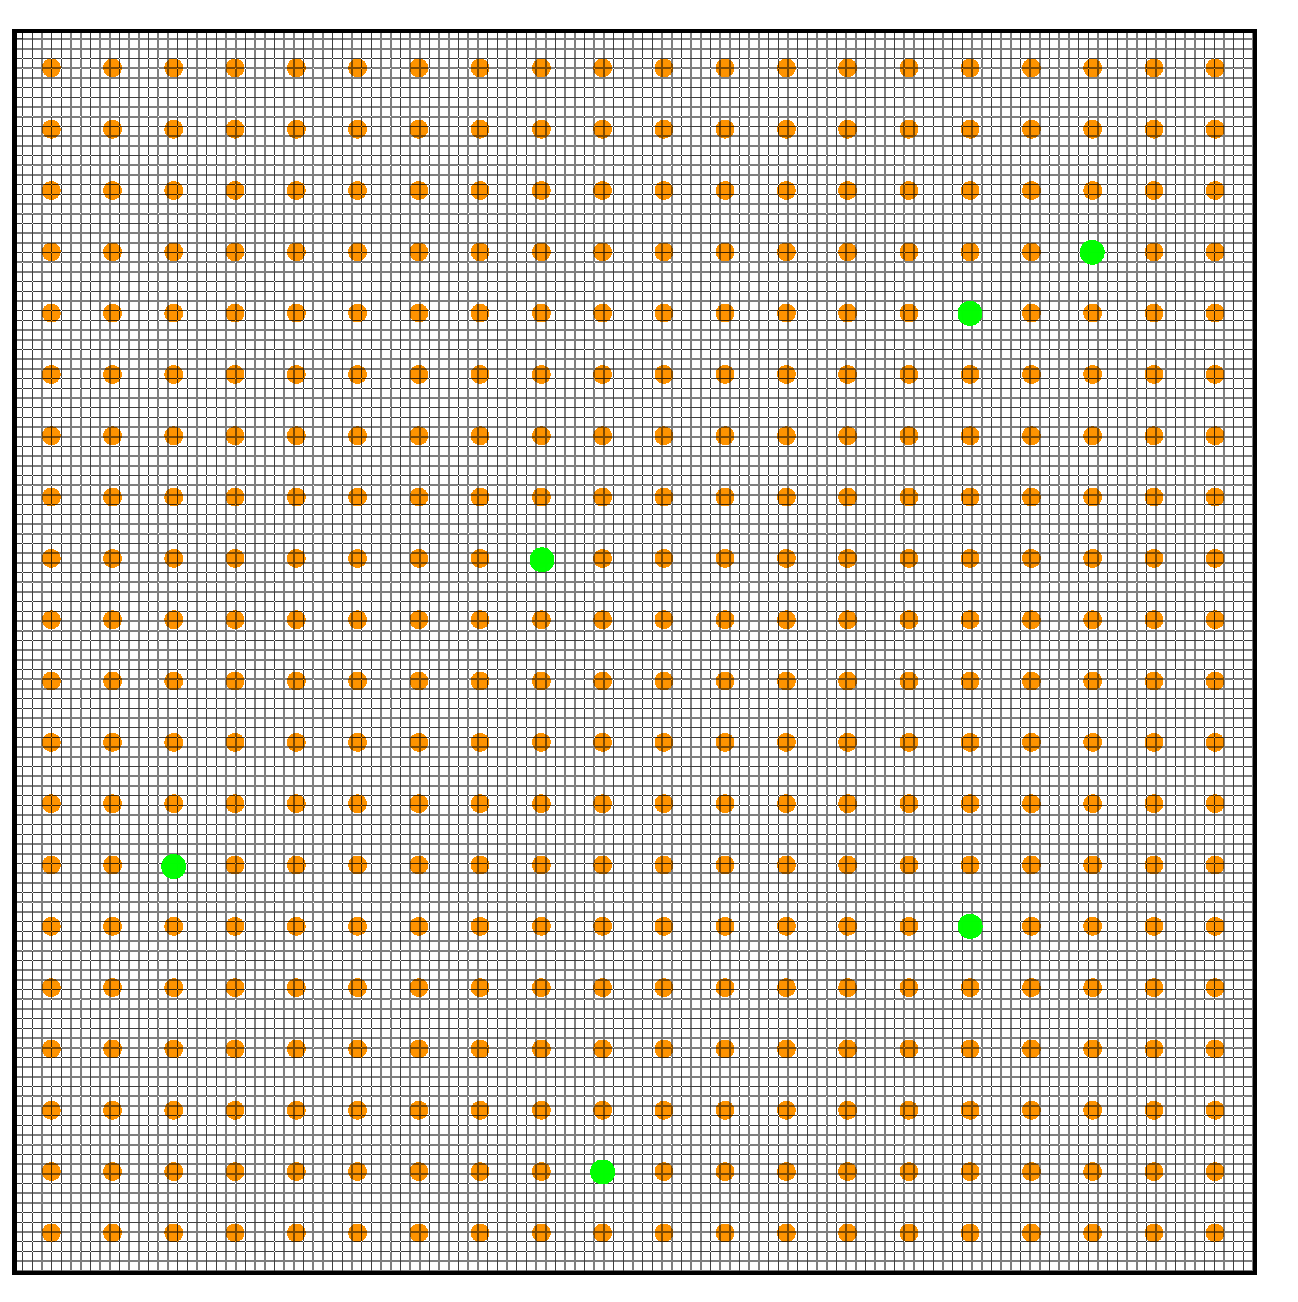
\includegraphics[width=\textwidth]{Ch5_QPIsim_demo.pdf}
	\caption[\textbf{schematics for the simulation}]{\textbf{schematics for the simulation}, in the actual calculation, we place defect at locations defined by lattice points indicated as green dots, and compute $\delta\rho(\textbf{x},\omega)$ at each spatial grid point (128 by 128 here)}
	\label{fig:ch5_qpisim_demo}
\end{figure}

\subsubsection{Simulation result}
A repository for \ac{LDOS} simulation on the model described above is made and shared on this \href{https://github.com/Plswearpants/QPI\_simulation}{github repository}.

The setup of simulation is illustrated in Fig. \ref{fig:ch5_qpisim_demo}, a grid of $128x128$ in real space covering a $20x20$ lattice space indicated in orange dots. We can implant defects on different lattice sites, indicated in green dots. 

\begin{figure}
	\centering
	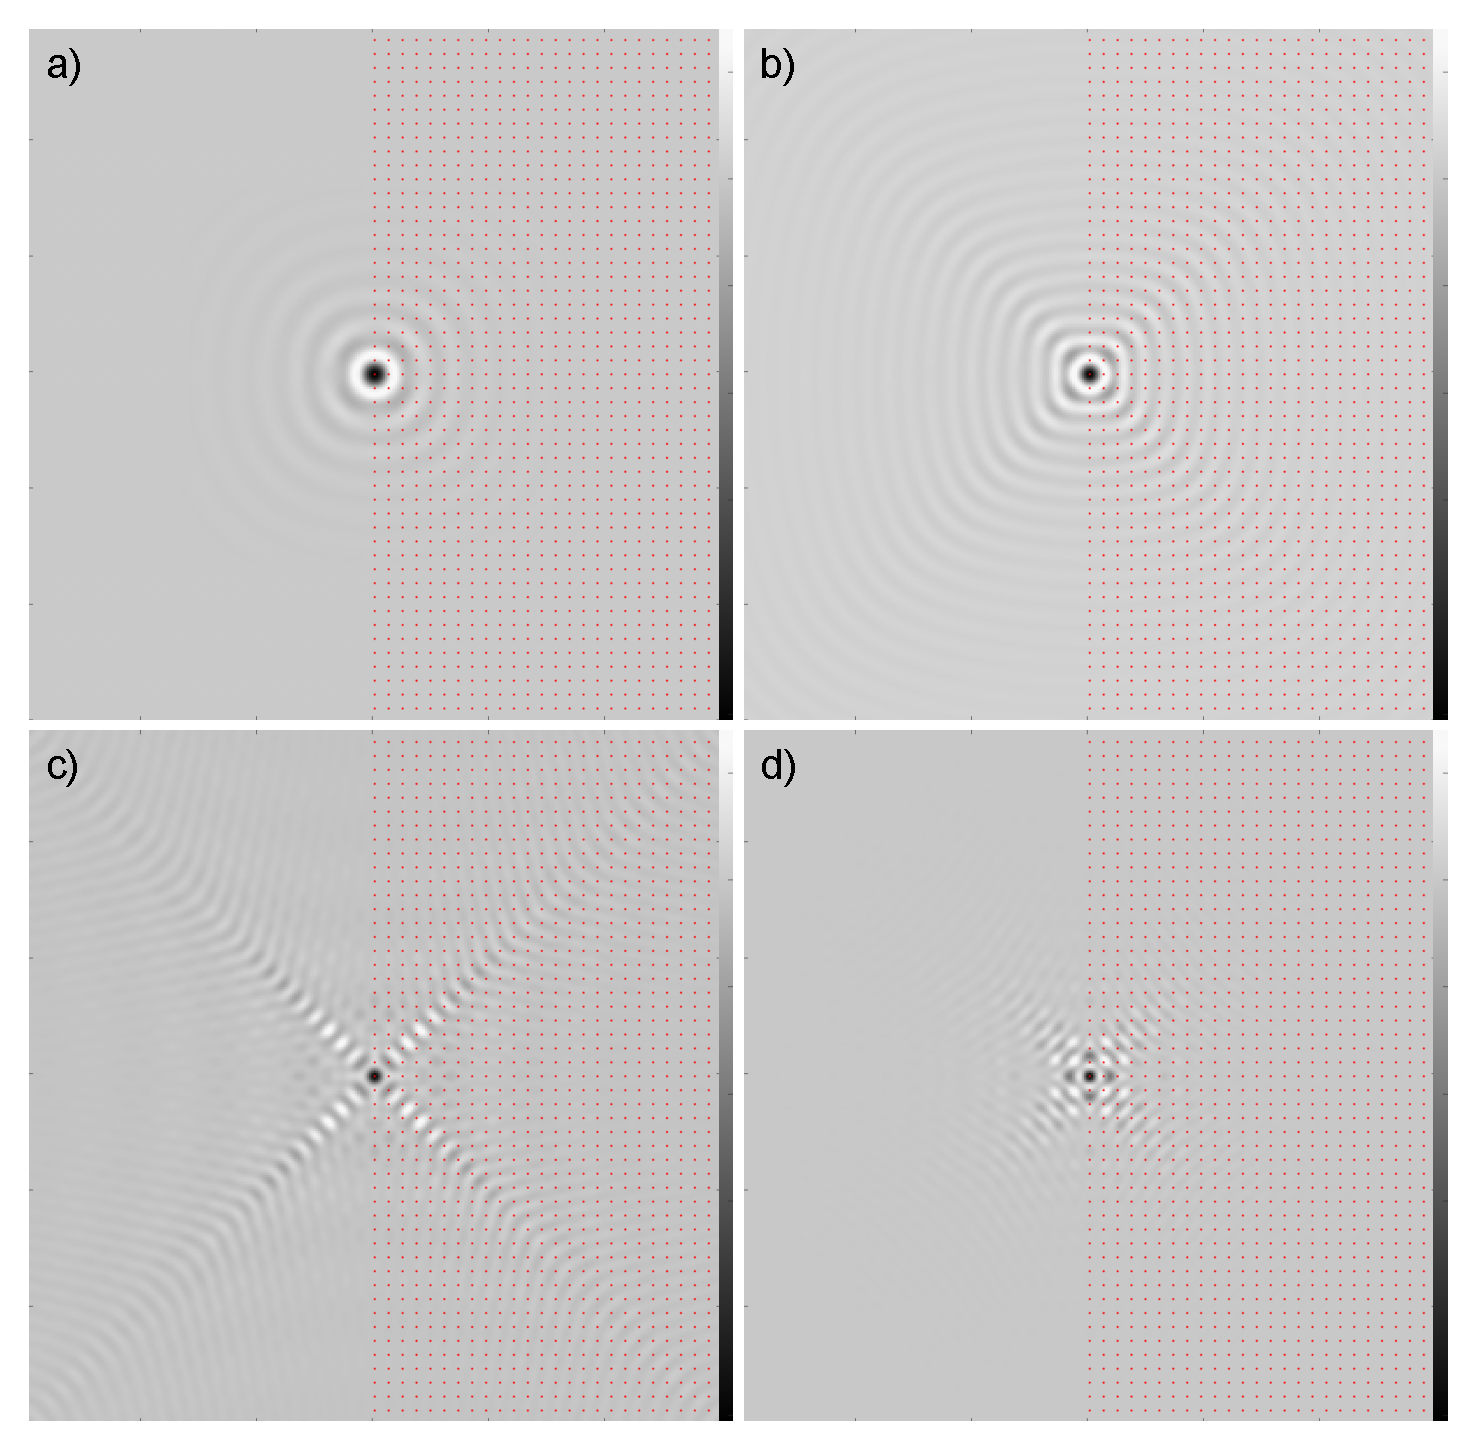
\includegraphics[width=\textwidth]{ch5_singe_simulation.pdf} % Replace with your image file
	\caption[\textbf{single defect QPI pattern simulation}]{\textbf{single defect QPI pattern simulation}: $\delta\rho(\textbf{x},\omega)$ for single defect at the center of the 51 by 51 lattice grid with t = -0.2 and $\omega$ = 0.45, 0.20, -0.05 and -0.45 eV for a)-d), respectively; the integrand size is defined by n = 300, $\epsilon = 1*10^{-3}$. Contrast for each image is self-normalized to [0,1].}
	\label{fig:ch5_single_scattering}
\end{figure}

We first performed a single defect calculation, where we place the defect at the center of a square lattice with $51\times51$ sites, $\delta\rho$ was numerically computed at a $301\times301$ grid chosen to overlap with the square lattice, with lattice parameter $a = 10^{-9}$, onsite energy $E_0 = 0$, defect energy $E_d=-0.02$, hopping parameter $t = -0.2$. In total, 41 energy slices are computed in an energy range of $(-0.5, 0.5)$eV.  

Typical \ac{LDOS} maps at different energy are shown in Fig. \ref{fig:ch5_single_scattering}, the figures are plotted on a gray scale image with the contrast indicating the level of \ac{LDOS} modulation. From the figures, we can make several observations:
\begin{itemize}
	\item The \ac{LDOS} modulation is featured by wave-like pattern similar to the Friedel oscillation, and the pattern varies with energy. 
	\item The wave pattern extends far into the space, we will show later that this indicating a relatively long life-time of this quasiparticle. 
	\item The wave pattern persists furthest in space near the Fermi level, at $E=-0.05eV$, the diagonal wave extended all the way to the boundary of the image, which correspond to a length of more than 25 lattice sites. 
\end{itemize}



\begin{figure}
	\centering
	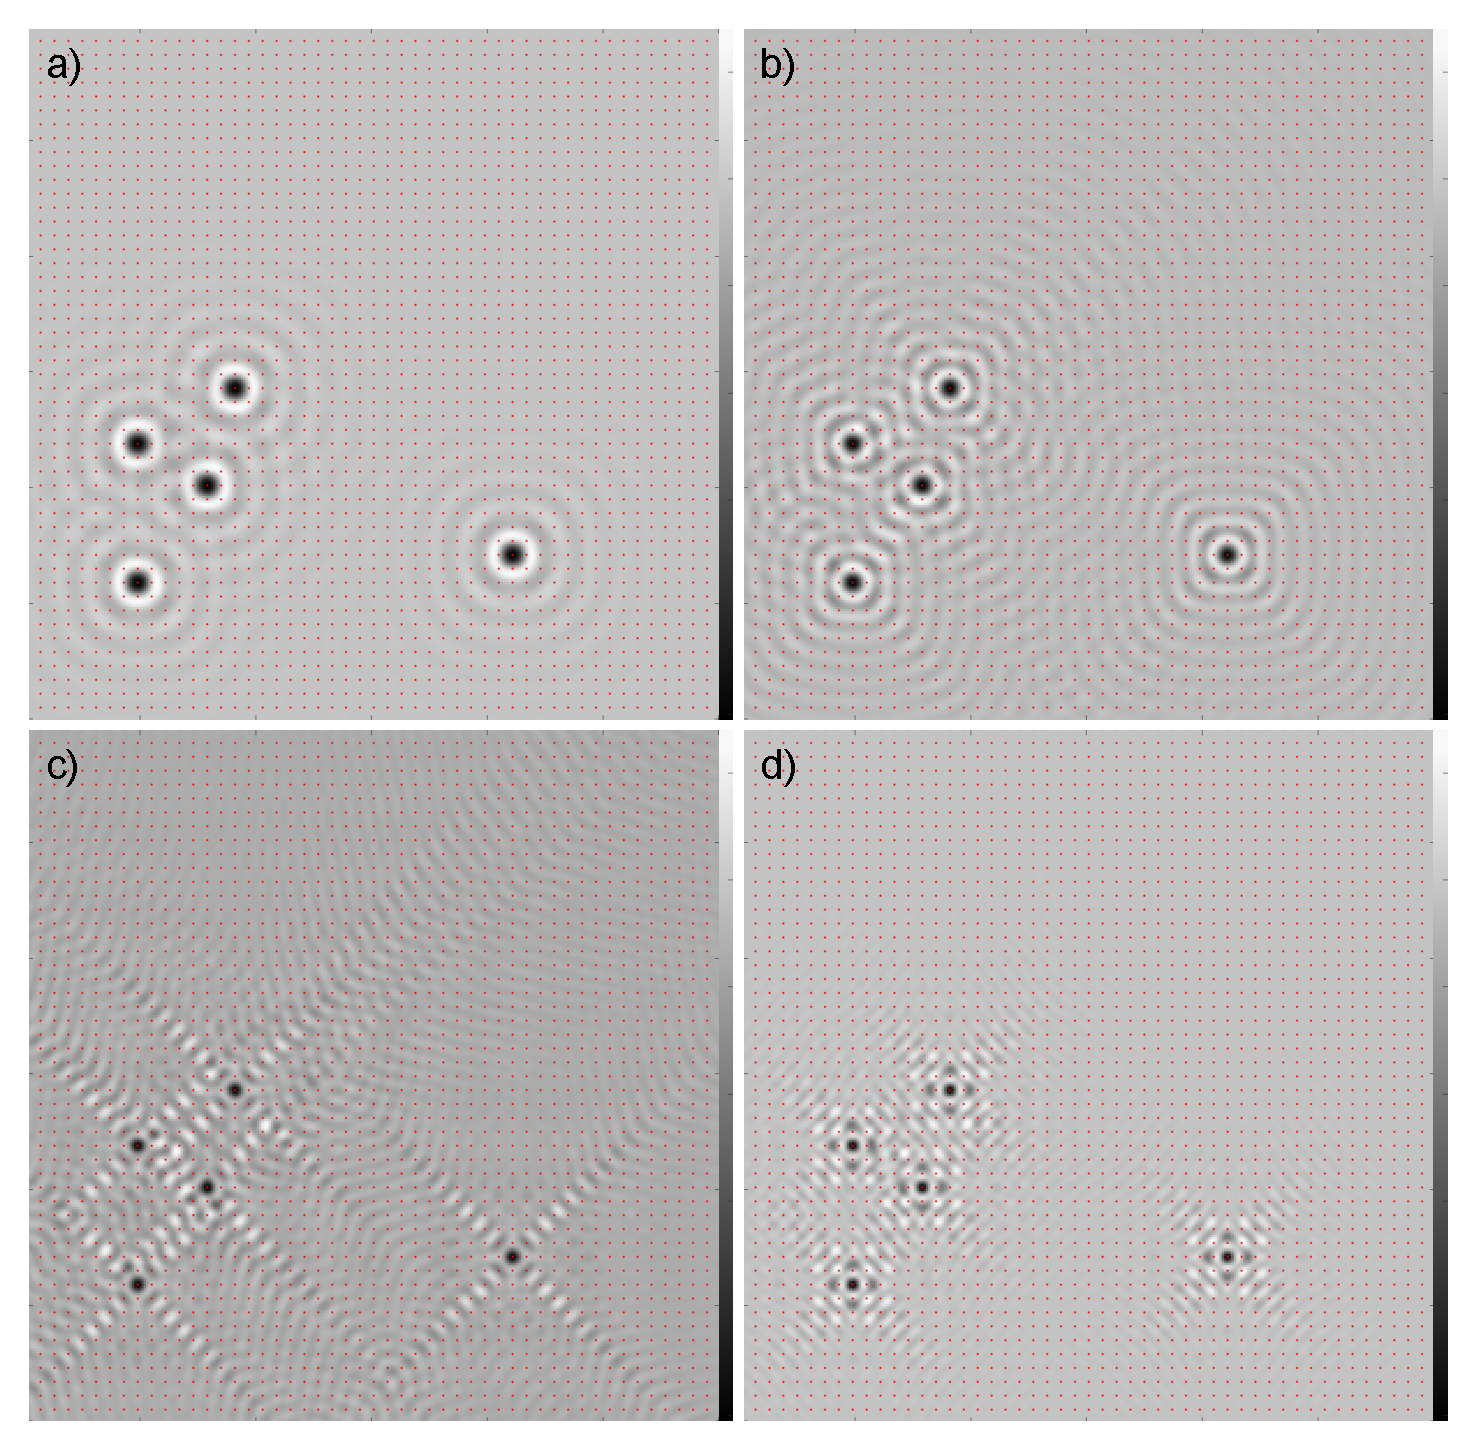
\includegraphics[width=\textwidth]{ch5_multi_simulation.pdf} 
	\caption[\textbf{Multi-defect QPI pattern simulation}]{\textbf{Multi-defect QPI pattern simulation}: $\delta\rho(\textbf{x},\omega)$ for 5 randomly placed defect on the 51 by 51 lattice grid with t = -0.2 and $\omega$ = 0.45, 0.20, -0.05 and -0.45 eV for a)-d), respectively; the integrand size is defined by n = 300, $\epsilon = 1*10^{-3}$. Contrast for each image is self-normalized to [0,1].}
	\label{fig:ch5_multi_scattering}
\end{figure}

We also calculated multi-defect results, for this, the T-matrix is no longer a scalar but rather a real matrix capturing the correlation between defects. Numerical results are calculated with Equation \ref{multi_defect_eq}, and shown in Fig. \ref{fig:ch5_multi_scattering}, where 5 defect locations are randomly selected on the lattice points. It is worth noting that multi-defect scattering calculation is relatively expensive as the size of T matrix grows as the square of defect numbers, later in Ch.5.3.2 we will show that we could approximate the multi-defect T matrix with only its diagonal terms with some corrections, making the calculation time linear with the numbers of defect.  
%we can see that the interference pattern from different defect sources are more prominent on spots with clustered defects. 


\subsection{Interpretation of QPI}\label{subsection: interpretationQPI}
Quasiparticle-impurity scattering gives rise to \ac{QPI}. Interpretations of \ac{QPI} can be quite involved in real materials, but all the factors to consider can be characterized into two aspects: 1. the details of quasiparticle states, and 2. the characteristics of the impurity. We will illustrate these aspects with the system we established for the simulation above. 

As mentioned at the start of Ch4.2, quasiparticles carry the same quantum numbers ($\textbf{k}$,$\sigma$) as the bare particles. Therefore, quasiparticles can be expressed by electronic states on the system's band structure. For the 2D Tight-binding model with only nearest-neighbor hopping that we considered, the energy dispersion $\epsilon_{\mathbf{k}}$ is a parabola in $k_x$ and $k_y$ as denoted in Equation \ref{E_k} and plotted in Fig. \ref{fig:ch5_bs} a). In an elastic quasiparticle-impurity scattering process, given our impurity is non-magnetic, we have the incoming state $\psi(\textbf{k}_i,\sigma)$ and outgoing state $\psi(\textbf{k}_f,\sigma)$, where $E_{\textbf{k}_f} = E_{\textbf{k}_i}$. To enforce elastic scattering, we can take a constant energy slice at a given energy; this reveals all possible states at that energy. This slice is normally referred to as a \ac{CEC} of that particular energy. While real-life materials can possess more complicated selection rules, in a single band situation as we formulated here, any state on the \ac{CEC} can be an initial or a final state in the scattering process. Mathematically, to describe the scattering vector $\textbf{q} = \textbf{k}_f -\textbf{k}_i$, we can take a self-convolution of the \ac{CEC}, which we can easily calculate and plot; This self-convolution is often referred as the \ac{JDOS} at the corresponding energy. An example is given at an energy close to the Fermi level in b),c) of Fig. \ref{fig:ch5_bs}. 
\begin{figure}
	\centering
	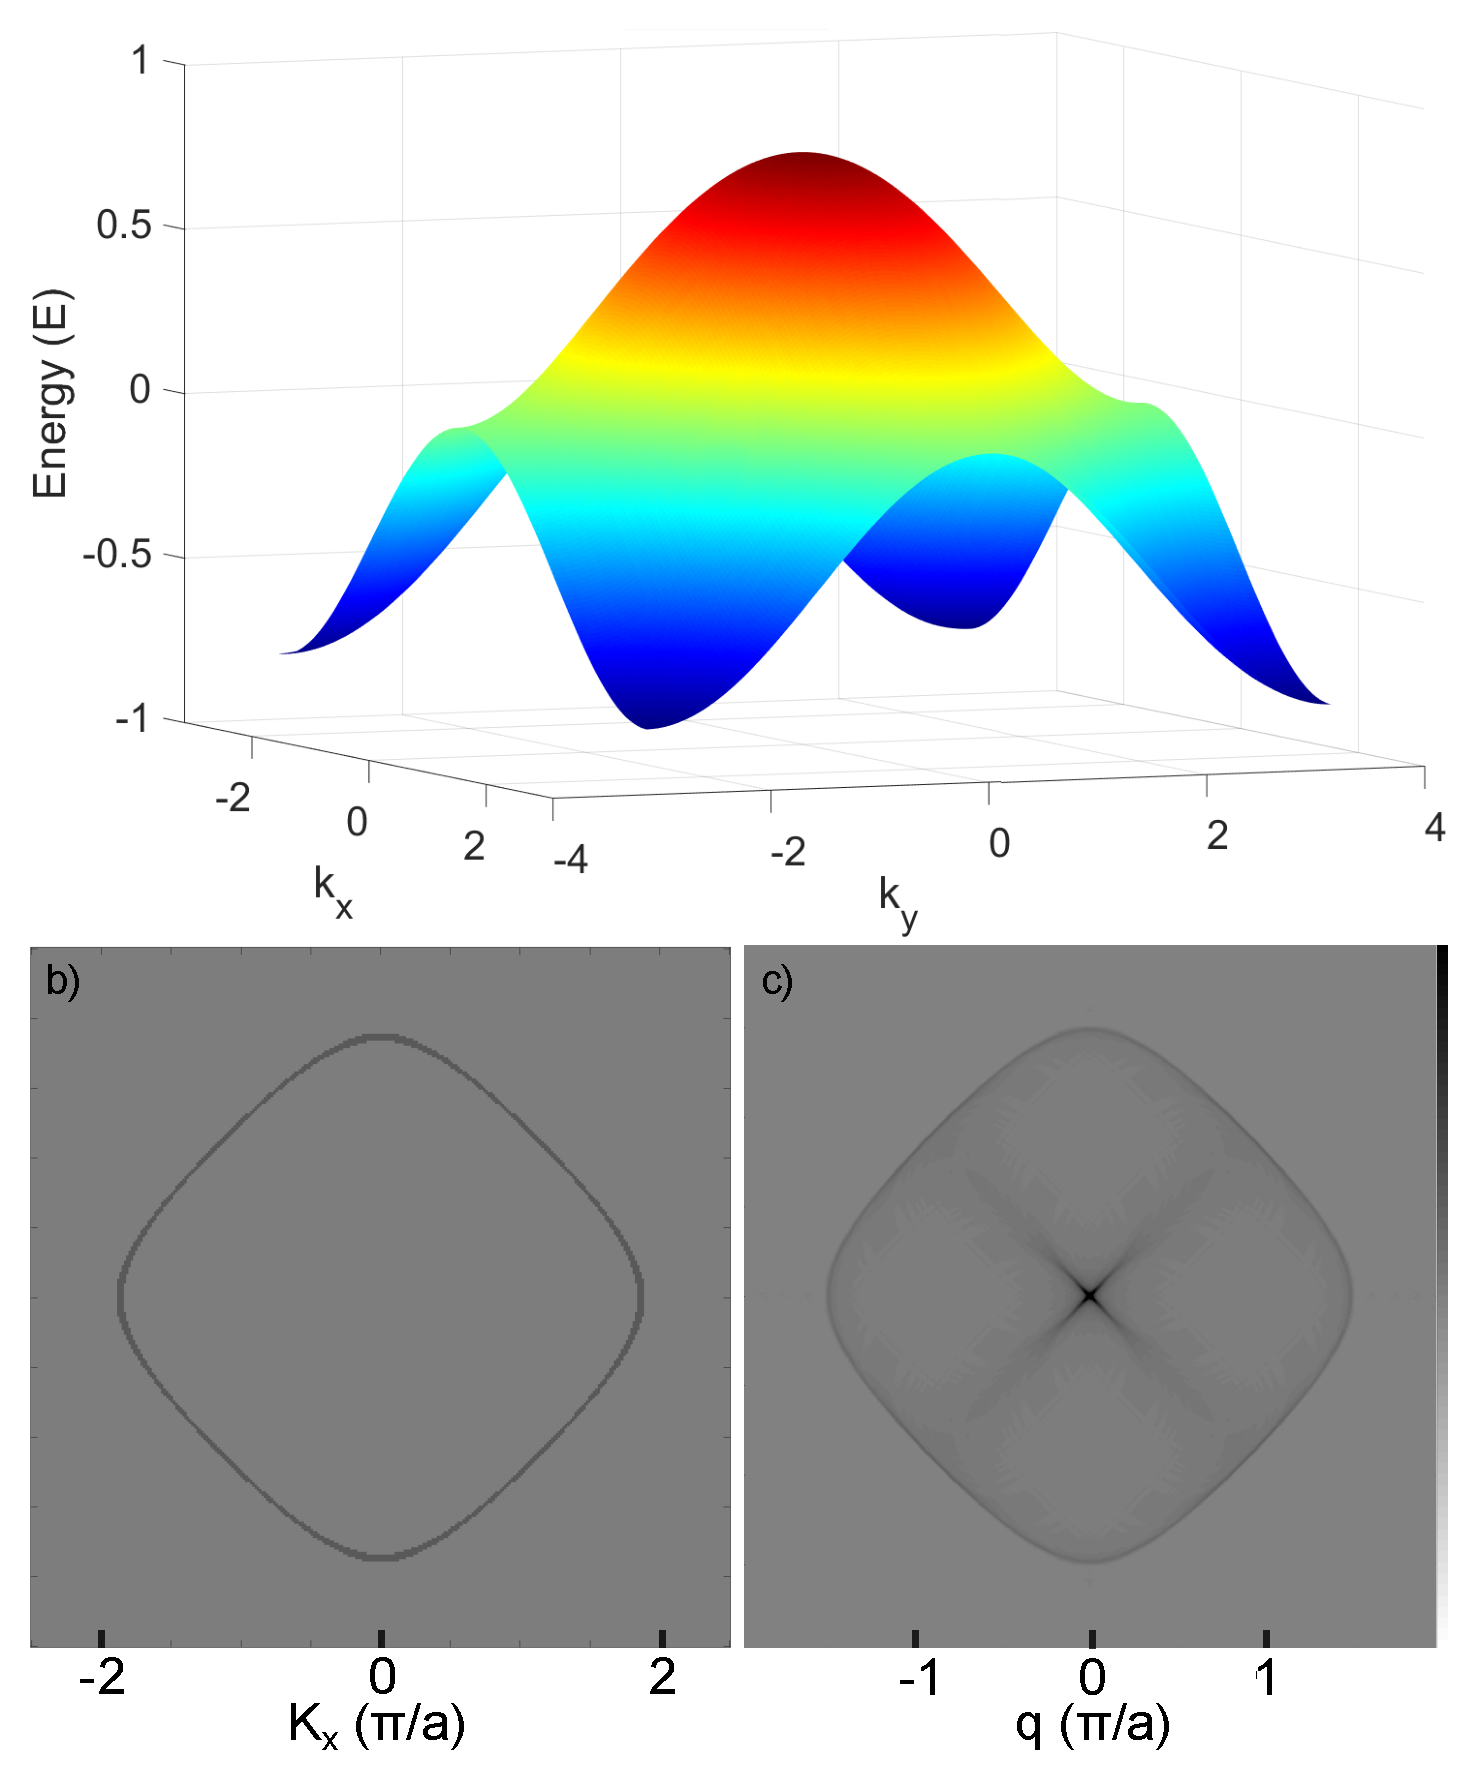
\includegraphics[width=\textwidth]{Ch5_BS_JDOS.pdf} 
	\caption[\textbf{Band structure of 2D tight-binding square lattice}]{\textbf{Band structure of 2D tight-binding square lattice with nearest neighbor hopping}: a) 3D Energy dispersion in $\textbf{k}_x$ and $\textbf{k}_y$, b) Constant energy contour and c) Joint density of states at $E=0.075eV$}
	\label{fig:ch5_bs}
\end{figure}

\begin{figure}
	\centering
	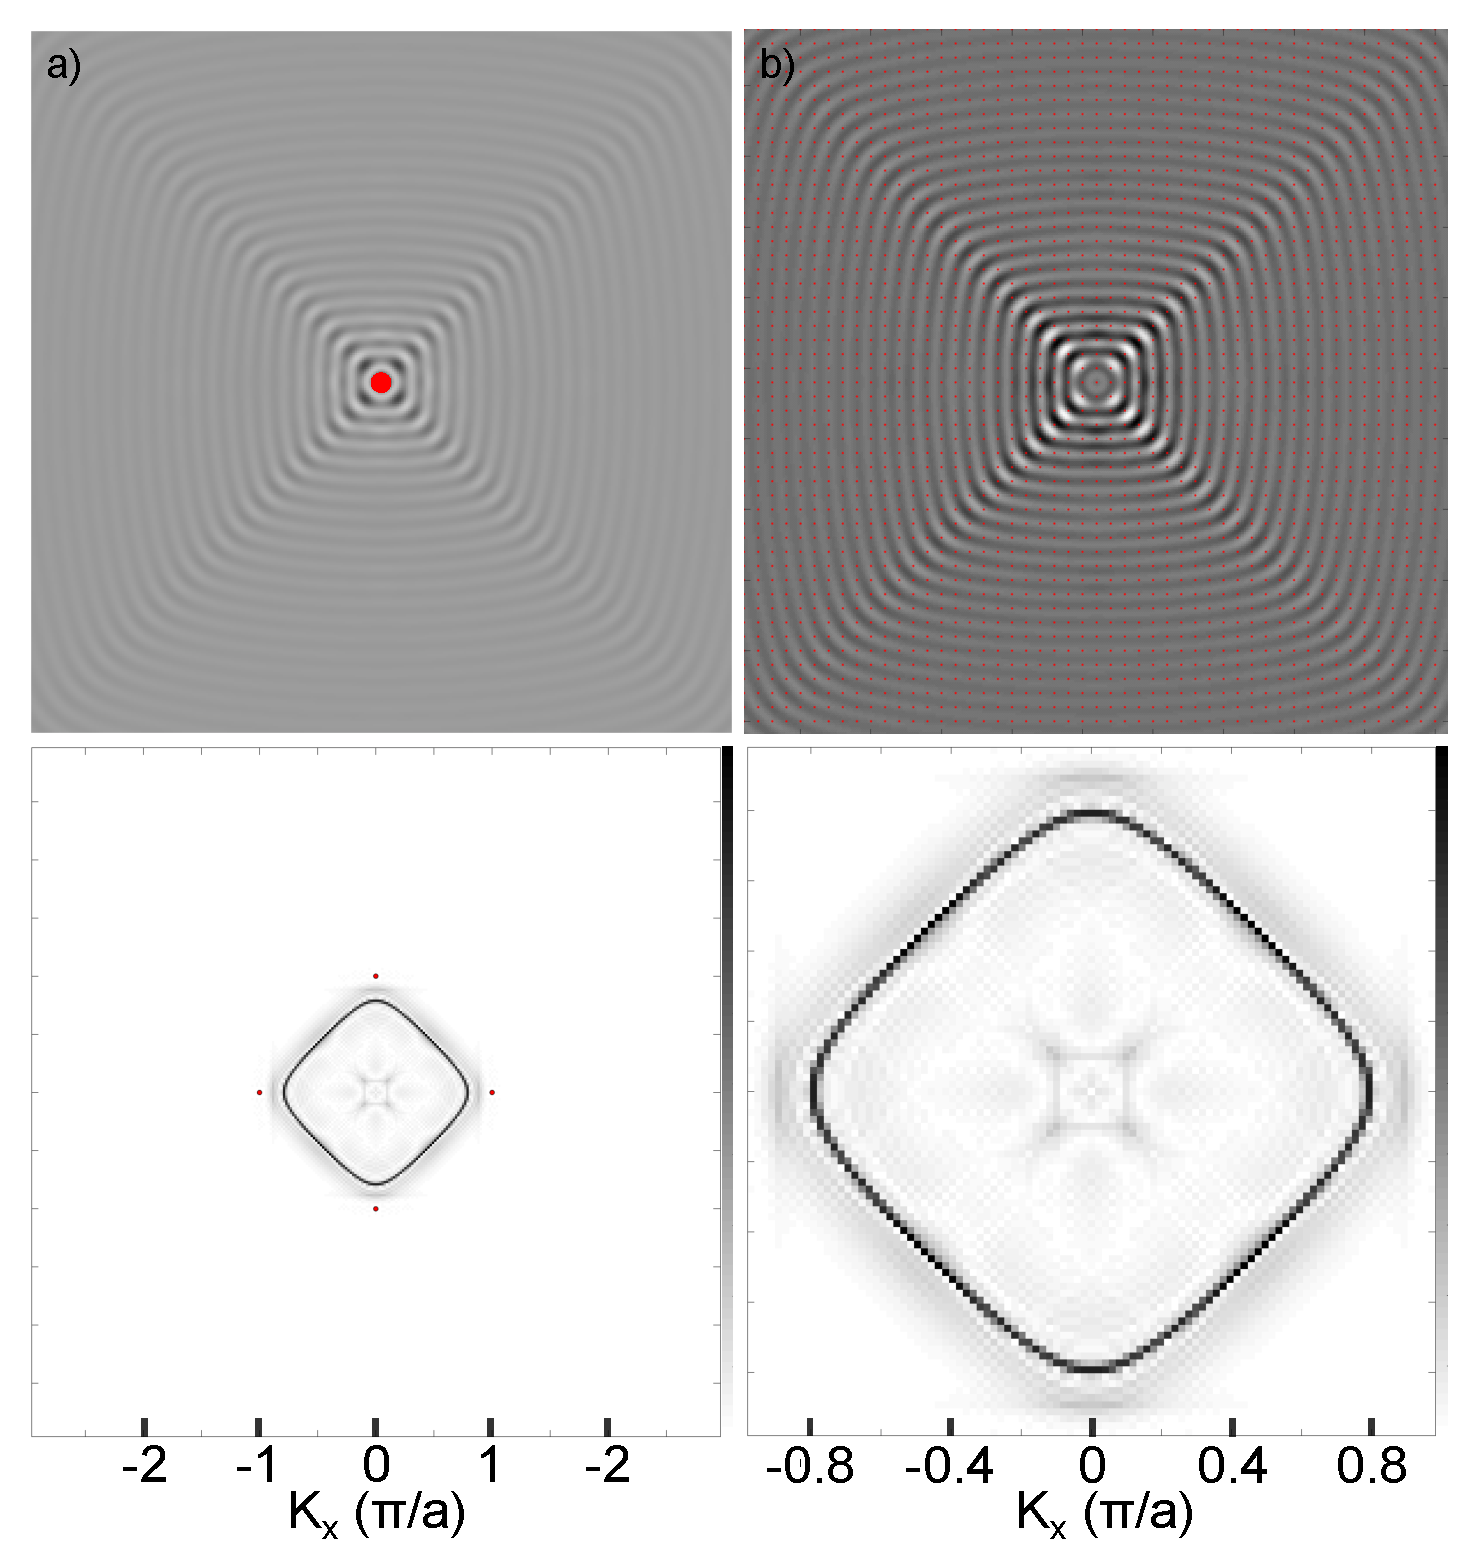
\includegraphics[width=\textwidth]{Ch5_LDOS_QPI.pdf} 
	\caption[\textbf{QPI pattern in both real-space and \textbf{q}-space}]{\textbf{QPI pattern in both real-space and \textbf{q}-space}. At $E=0.075eV$, we first suppress the defect feature with a Gaussian mask at the red dot in a), this gives us b). We then apply 2D Fourier transformed to b) and get c); the red dots are indications of the Bragg peaks of the square lattice. d), \textbf{q}-space QPI map cropped within the Bragg peaks for better visibility of low-\textbf{q} features}
	\label{fig:ch5_ldos}
\end{figure}

The real space \ac{LDOS} modulation can now be interpreted, and we illustrate it with Fig. \ref{fig:ch5_ldos}. First, to focus on the interference ripples, we suppress the features from the defect itself by applying a Gaussian mask at the defect location, a)-b). Then, we apply the Fourier transform and take the power spectrum to get the \ac{QPI} map in reciprocal space as shown in c); the red dots in c) are the Bragg peaks of the system. Encoded with Fourier transform, the range in reciprocal space is inversely proportional to the real space resolution. High $\textbf{q}$-space features correspond to high-frequency features in the real space, and in most cases, scattering vectors are confined in first Brillouin zone. However, there are cases like Umklapp scatterings that presents wavevectors that extend beyond the Bragg peaks, these features are usually low in intensity as they are second-order(or more) effect. Therefore, a common practice is to truncate and keep the feature within the Bragg peaks; this gives us a closer look at the features, as shown in d). You might be wondering why then we take grid map with spatial resolution denser than the lattice parameter; This is because for the reason given Nyquist–Shannon Sampling Theorem, we need to take grid fine enough to see the Bragg peaks; Thus, in practice, we take at least two pixels per lattice site in each direction.  

We now take a closer look at how the scattering wave vectors manifest in real and momentum spaces. As shown in Fig \ref{fig:ch5_compare}, we first measured the real-space wavelength $\lambda_d$ and $\lambda_h$ on the diagonal and horizontal direction, respectively; We then transfer the wavelength into \textbf{q}-space and draw the corresponding $\textbf{q}_d$ and $\textbf{q}_h$ in b). By transferring them one to one into the \ac{CEC} in c), we can map two sets of initial and final momentum states. For each $\textbf{q}$-vector, we have $\textbf{q} = \textbf{k}_2 - \textbf{k}_1$ and the corresponding scattering vector can also be found in the \ac{JDOS} at the same energy. 
\begin{figure}
	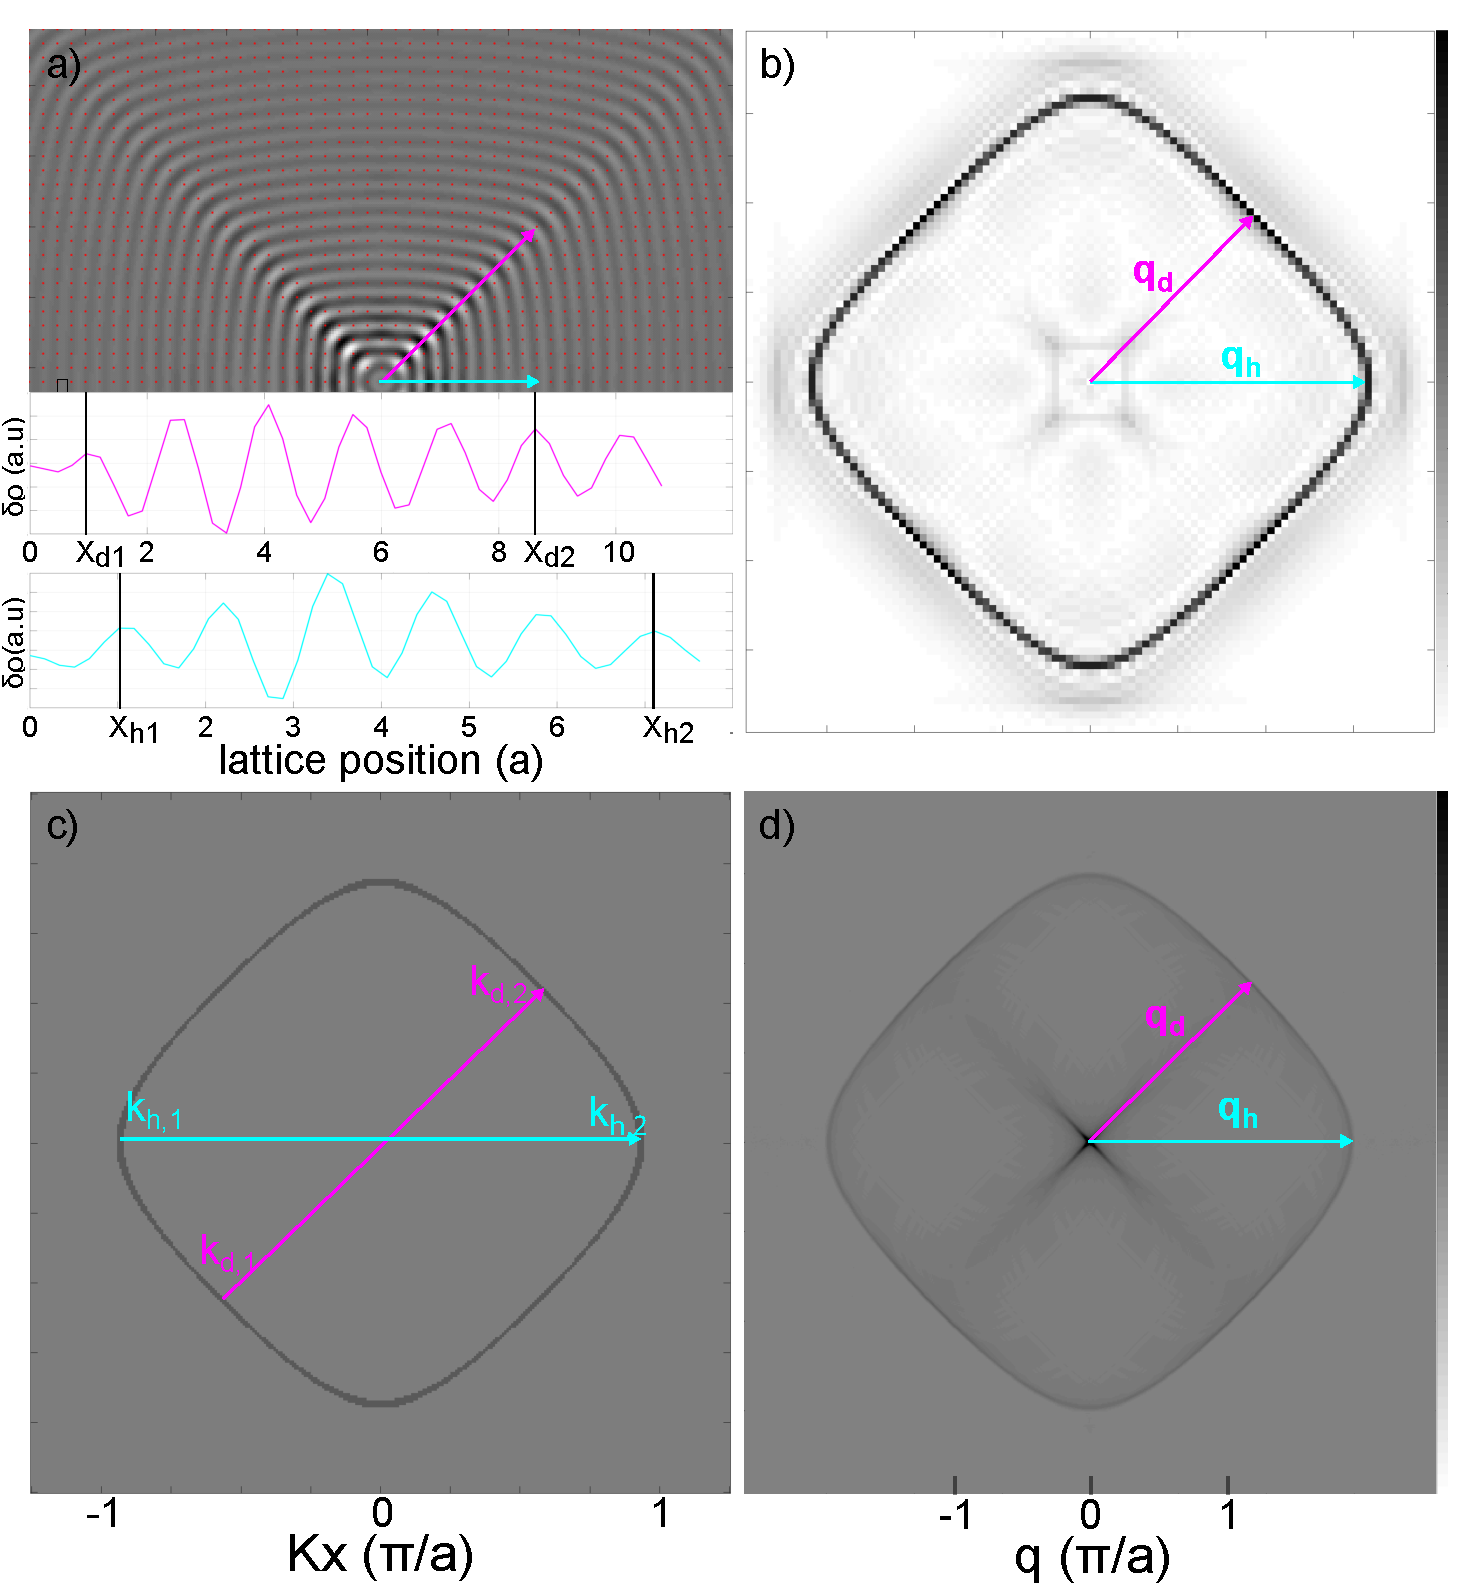
\includegraphics[width=1.1 \textwidth]{Ch5_QPI_JDOS.pdf} 
	\centering
	\caption[\textbf{Illustration of scattering vectors in both real-space grid map and \textbf{q}-space QPI map, and comparison with the band structure and JDOS}]{\textbf{Illustration of scattering vectors in both real-space grid map and \textbf{q}-space QPI map, and comparison with the band structure and JDOS}. a) horizontal(colored in cyan) and diagonal(colored in magenta) profile on the grid map, the real space wavelengths $\lambda$s are calculated by mapping the peaks in profile as shown in the insets, $\lambda_d = \frac{X_{d2}-X_{d1}}{5} \approx 1.53 a$, $\lambda_h = \frac{X_{h2}-X_{h1}}{5} \approx 1.21 a$. We then draw these 2 vectors in \textbf{q}-space in b), we can see the 2 corresponding vectors points at the high-intensity contour. We then transfer these 2 vector \textbf{k}-space in c) and we found that they corresponds to states on the \ac{CEC}, which correspond to the same \textbf{q}-vectors in the \ac{JDOS} in d).}
	\label{fig:ch5_compare}
\end{figure}

There are two features in $\textbf{q}$-space \ac{QPI} that are worth mentioning: First, nested \ac{CEC} creates more concentrated intensity in $\textbf{q}$-space \ac{QPI}. Nesting is a Fermiology term that refers to situations where relatively large portions of the Fermi surface (or \ac{CEC}) can be connected by the same scattering wavevector \textbf{q}; As many initial and final states differ by the same wavevector, the scattering is strongly enhanced at that wavevector. This results in high \textbf{q}‐space overlap and thus one observes strong intensity (peaks) at the nesting wavevectors. 

In a two-dimensional system, a \ac{CEC} is nested when we have pairs of lines that have the same separation. A schematic is shown in Fig. \ref{fig:ch5_schema_nesting} to illustrate the  nesting effect, for a square \ac{CEC}, scattering between many states on the parallel lines can be described by the red arrows, and in b), the log-scale self-convolution of a), this correspond to the intensity concentration at the red arrow. While for a circle like c), nesting is not presented, and thus the intensity of the self-convolution map d) is more spread. This can also be seen in the simulation data as shown in Fig. \ref{fig:ch5_nest}; a) and c) are 2 \ac{CEC} at two different energies that present different shapes. Compared with the circle-like shape c), a) can be approximated as a square, and thus has a more concentrated intensity in the corresponding \textbf{q}-space QPI map.

\begin{figure}
	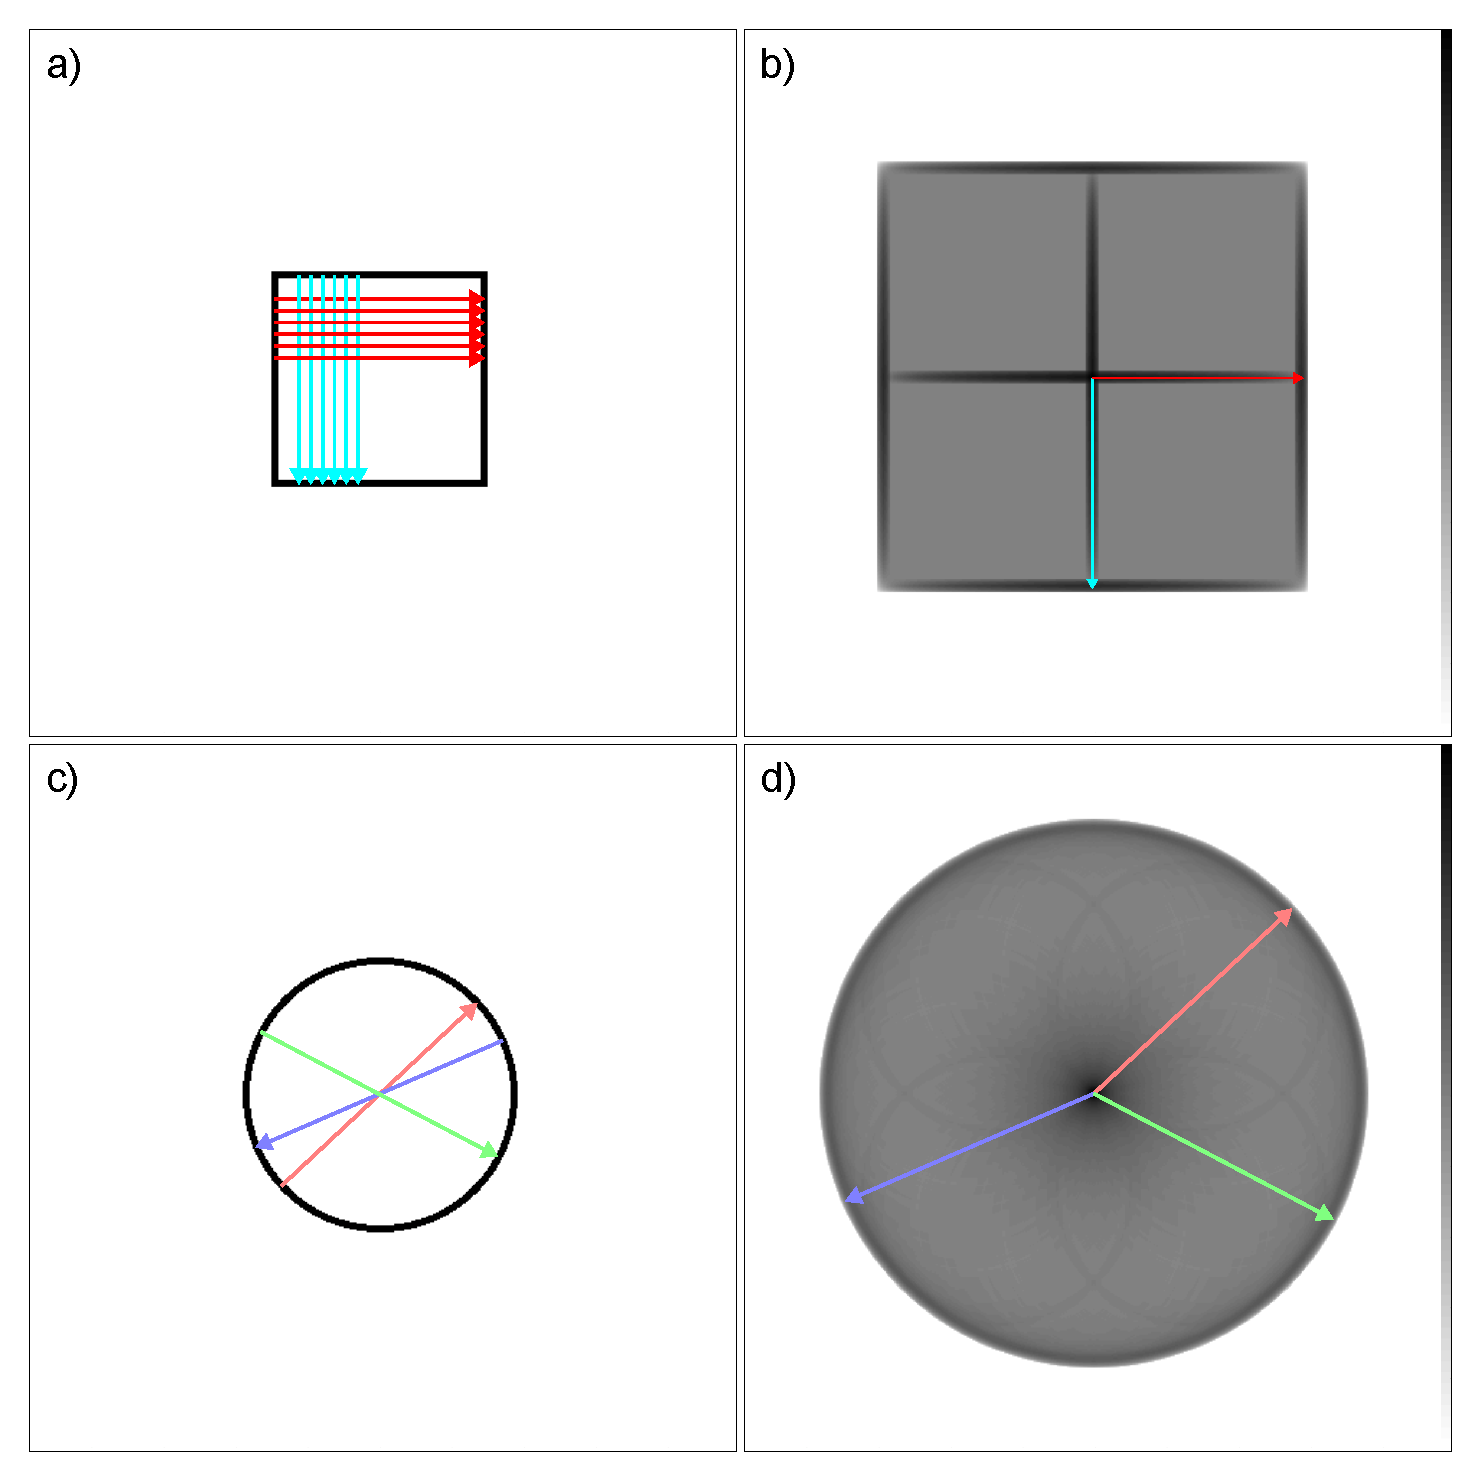
\includegraphics[width= \textwidth]{Ch5_nesting_schematic.pdf} 
	\centering
	\caption[\textbf{Schematics of the nesting effect}]{\textbf{Schematics of the nesting effect}. a),c) are two schematic \ac{CEC}s with different shapes; black pixels represent the occupied states, number of states on a) and c) are made the same as ensured by the same circumferences. b) and d) are corresponding log-scaled \ac{JDOS}, with clear difference in the spread of the intensity, b) has a much concentrated intensity due to nesting compared to d).}
	\label{fig:ch5_schema_nesting}
\end{figure}

\begin{table}
	\centering
	\begin{tabular}{|c|c|c|c|}
		\hline
		Energy (eV) & Width ($\pi/a$) & Width Uncertainty ($\pi/a$) & R-squared \\
		\hline
		-0.5 & 0.0661 & 0.0044 & 0.9689 \\
		-0.4 & 0.0496 & 0.0040 & 0.9715 \\
		-0.3 & 0.0383 & 0.0034 & 0.9724 \\
		-0.2 & 0.0300 & 0.0028 & 0.9767 \\
		-0.1 & 0.0274 & 0.0032 & 0.9814 \\
		\hline
		0.075 & 0.0201 & 0.0014 & 0.9964 \\
		0.1 & 0.0309 & 0.0120 & 0.8943 \\
		0.125 & 0.0214 & 0.0013 & 0.9958 \\
		0.2 & 0.0286 & 0.0065 & 0.9350 \\
		0.3 & 0.0311 & 0.0048 & 0.9635 \\
		0.4 & 0.0392 & 0.0051 & 0.9544 \\
		0.5 & 0.0516 & 0.0062 & 0.9451 \\
		\hline
	\end{tabular}
	\caption{Horizontal profile fitting results showing the width and its uncertainty (in units of $\pi/a$) along with the R-squared values for both positive and negative bias energies.}
	\label{tab:qpi_fit_results_combined}
\end{table}

Secondly, the quasiparticle lifetime decreases as we move away from the Fermi surface. Given the momentum dependence of $\operatorname{Im}{\Sigma_{\textbf{k},\sigma}(\omega+i \eta)}$ is negligible, which is usually true, the spectral function is a simple Lorentzian in $\textbf{k}$-space of width $\operatorname{Im}{\Sigma}$ \cite{wolfleQuasiparticlesCondensedMatter2018}; Therefore, the \textbf{q}-space quasiparticle peak is also a Lorentzian with its width approximated at 2$\operatorname{Im}{\Sigma}$. Note that $\operatorname{Im}{\Sigma}$ is inversely proportional to the quasiparticle lifetime $\tau_{QP}$; thus, we can probe $\tau_{QP}$ by analyzing the broadening of the quasiparticle peaks in $\textbf{q}$-space \ac{QPI} at different energies, similar to what this literature did\cite{grotheQuantifyingManyBodyEffects2013a}. As shown in \ref{fig:ch5qplifetime}, we first take a horizontal line profile on the \textbf{q}-space \ac{QPI} that goes through the center, then fit a Lorentzian function on the quasiparticle peak region shown in the green dots in b), we can extract the peak width with its uncertainty. We then apply this process through different energy slices; the results are presented in Table \ref{tab:qpi_fit_results_combined} and plotted in c) of Fig. \ref{fig:ch5qplifetime}. All fittings possess an R-square value greater than 0.90 except for $E=0.1$; we thus marked the datapoint red in the plot. Quasiparticle peaks broaden as the energy deviated from the Fermi energy; however, within the energy range investigated, we still observe very sharp quasiparticle peaks, indicating long-lived and well-defined quasiparticles. 



\begin{figure}
	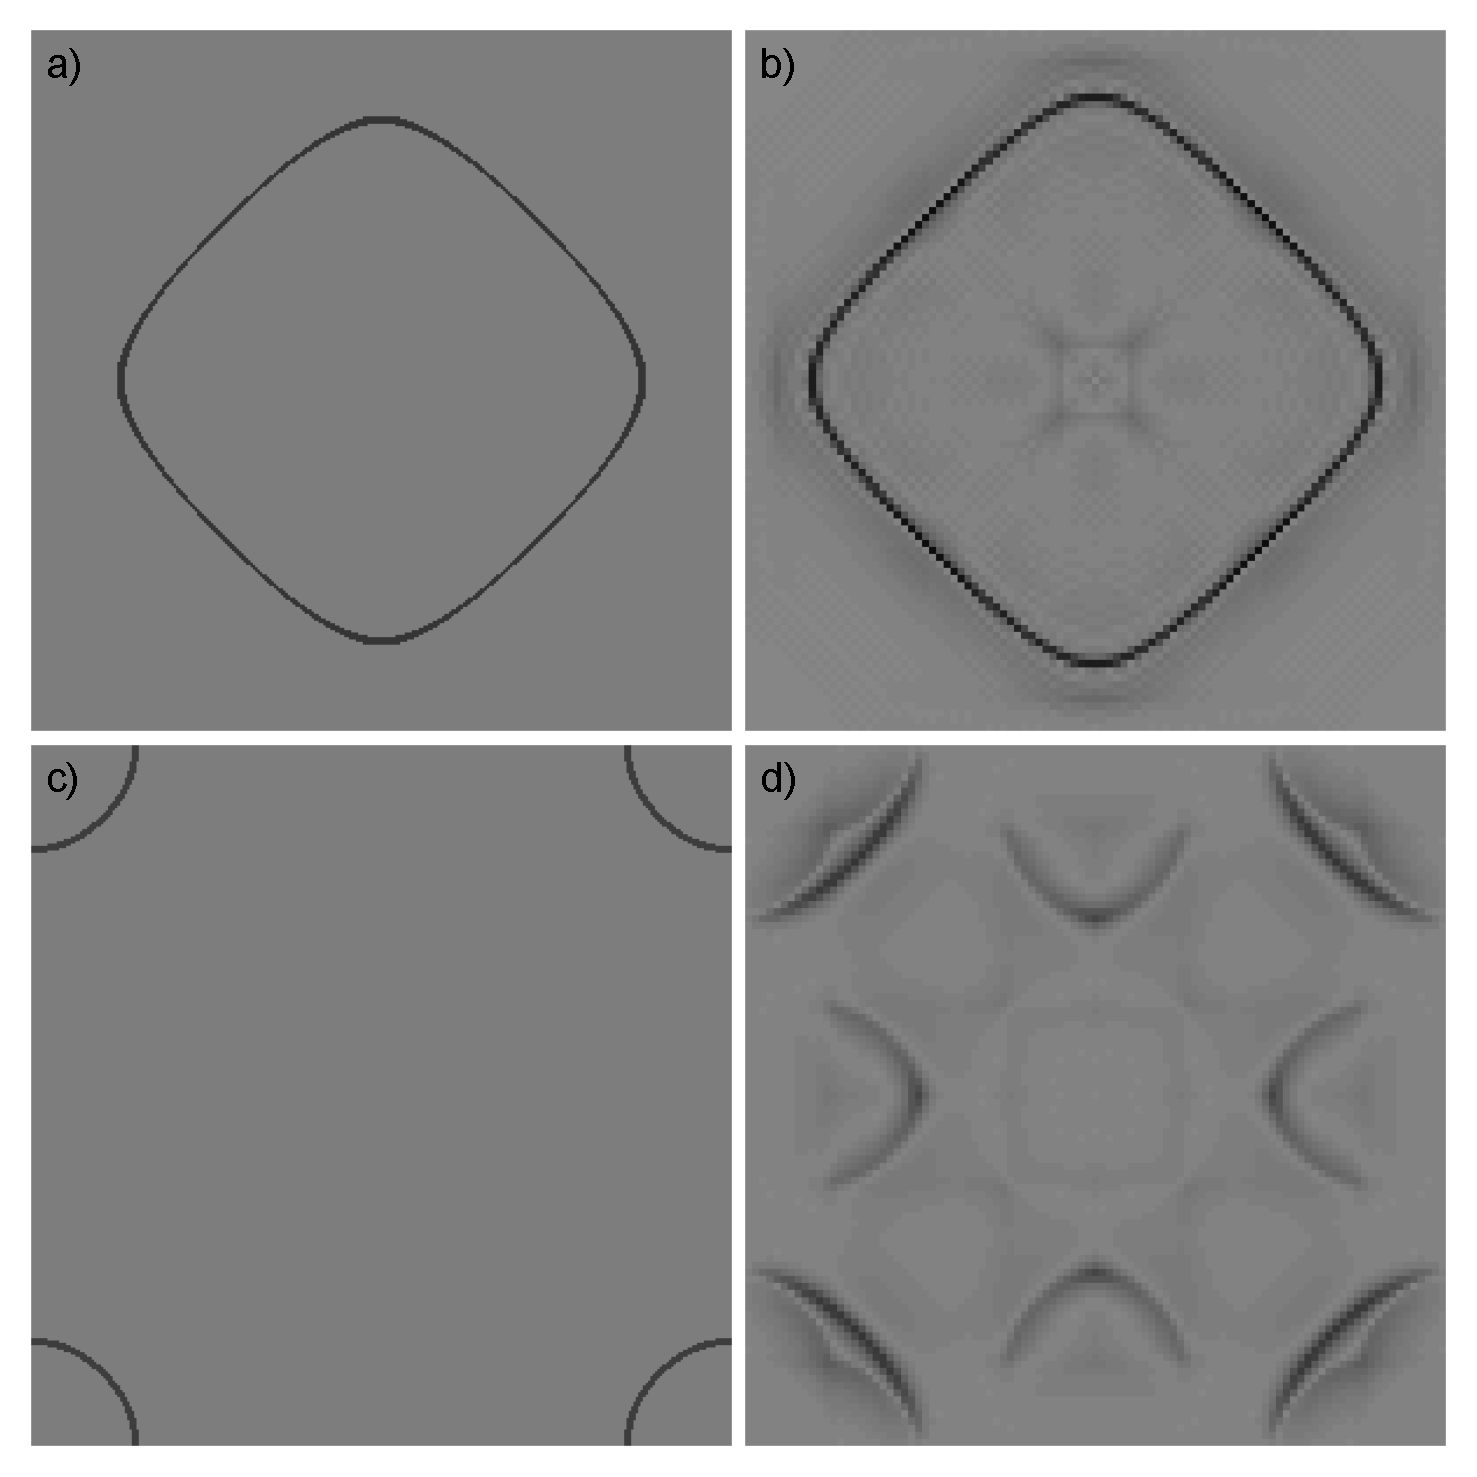
\includegraphics[width=\textwidth]{Ch5_nesting.pdf} 
	\centering
	\caption[\textbf{Comparison of nesting effect on \ac{CEC} with different shapes}]{\textbf{Comparison of nesting effect on \ac{CEC} with different shapes} Nesting is presented in the square-like \ac{CEC} a), and gives a more concentrated intensity in the QPI map b). While a circle-like \ac{CEC} like c) gives a more spread out the intensity in d).}
	\label{fig:ch5_nest}
\end{figure}


\begin{figure}
	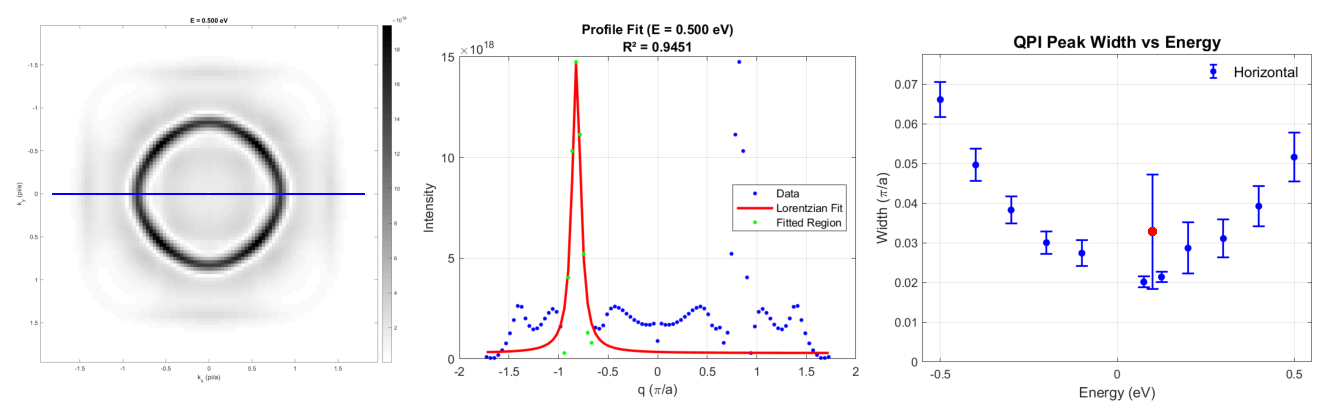
\includegraphics[width=\textwidth]{Ch5_qp_lifetime.pdf} 
	\centering
	\caption[\textbf{Quasiparticle lifetime decay}]{\textbf{Quasiparticle lifetime decay}. Fitting quasiparticle peaks with Lorentzian and extracting the width at different energy levels. a)-b) For an illustration of the process, we first extract the horizontal profile of the QPI map; then, we identify two peaks in the profile; by symmetry argument, we fit one peak with the Lorentzian function. c) QPI peak width across different energies, we see that as energy moves away from the Fermi level, the peaks broaden and $\tau_{QP}$ decreases. Data point at E = 0.1eV is marked red for its bad fitting quality according to R-square value in Table 4.1.}
	\label{fig:ch5qplifetime}
\end{figure}
%todo: maybe we can talk about the phase effect from impurity configuration. 


%Estimating the multidefect result with convolution approach inherently makes assumption into the independent nature of scattering, which is only true for weak scattering and sparse impurity distributions. 

Finally, different defect configurations produce distinct \ac{QPI} fingerprints because each defect acts as a scattering interface that imparts a characteristic phase shift to the quasiparticle wavefunction. In the T-matrix formalism, this effect is encoded in the complex scattering matrix element $M_{\mathbf{k,k'}}= \braket{\psi_\mathbf{k}|V_d|\psi_\mathbf{k'}}$, where the defect potential $V_d$ captures the real-space configuration of a defect. Similar to how a photon picks up a phase when reflected off an interface, the outgoing electronic state also gain a phase shift. 
This phase shift is different from the relative phase contained in the incoming and outgoing Bloch wave functions:
\begin{align}
	\ket{\psi_{\mathbf{k}}} &= e^{i\mathbf{k}\cdot \mathbf{r}} u_{\mathbf{k}}(\mathbf{r}),\\
	\ket{\psi_{\mathbf{k'}}} &= e^{i\mathbf{k'}\cdot \mathbf{r}} u_{\mathbf{k'}}(\mathbf{r}),
\end{align}
which arises from lattice symmetry, orbital character, spin texture, Berry phase and other characteristics of the band structure. 

When the phase shift introduced by a given defect mismatches, or resonances with the intrinsic phase relation between certain initial and final states, the corresponding QPI channels can be either suppressed or enhanced. Consequently, different defect configurations—through their distinct potentials and associated phase shifts—modulate QPI intensities in unique ways, providing the microscopic basis for defect-specific interference patterns.

\section{Experimental QPI measurement}
Real space \ac{QPI} signals are obtained by taking the grid map experiment on a region that presents \ac{QPI} patterns. In this section we will briefly explore \ac{QPI} measurements in the \ac{STM} experiment, more specifically, we will introduce the factors that dictate \ac{QPI} quality, discuss how to choose proper parameters that result in a good \ac{QPI} measurement, and finally we will present a specific challenge called the phase noise, which motivates our work in the next chapter.


\subsection{QPI measurement and quality}
As mentioned in Ch.2, taking a grid map is very involved. A successful grid map requires both an ideal instrumental setup and a set of proper measurement parameters based on the understanding of the target material. 

The key objective of an ideal instrumental setup is to create a stable environment and lower the system noise; as we discussed in Ch.2, this involves minimizing the noise from mechanical vibration, temperature fluctuation, and electronic instability of the system and maintaining a stable tip-surface tunneling junction. 

A grid map is defined by a $N\times N$ (assuming square) grid on a targeted area of $L \times L$ $nm^2$, this provides a spatial resolution $\Delta L = \frac{L}{N}$; In reciprocal space, this set up gives a range $Q = \frac{2 \pi}{\Delta L}$ with resolution $\Delta Q = \frac{2\pi}{L}$, the energy range and resolution is defined by the setting of the single-point spectroscopy performed on every grid point. 

A set of proper parameters for \ac{QPI} measurement aims to extract the most amount of information with the highest level of resolution given the constraints of the system. The most important constraint is the cryogenic hold time. This puts a ceiling on the grid map run time, while different systems vary; typically, the cryogenic holding time is a a few days to a week; for the machine used in this study, the holding time is half a week. Within the boundary of the run time, we usually aim for a grid with a fine reciprocal resolution $\Delta Q$ and a reasonable reciprocal range $Q$, corresponding to a large field of view $L$ and a reasonable $\Delta L$. It is intuitive to have a proper size of reciprocal range $Q$ that is not infinitely large, as most of the q-space features reside within the Bragg peaks, exemplified by Fig. \ref{fig:ch5_ldos} c). But we also do not want the field of view $L$ to be too large, this is because in real experiments with finite noise level, the featured \ac{QPI} pattern has a finite lifetime and its intensity will dive under the noise at some cutoff distance $r_{cutoff}$ from the defect center; Thus, a field of view larger than the cutoff distance will instead decrease the signal to noise ratio. We illustrate cutoff distances in systems with different noise levels in Fig. \ref{fig:ch5_cutoff}. The noise level is set to be noiseless, SNR = 10, and SNR = 1.2, respectively; given the noise level shown in the green dotted line, we identify the furthest signal peak higher than the noise level and place a blue vertical line there. These vertical lines indicate the cutoff distances; and we can see with increasing noise level, $r_{cutoff}$ drops, and thus the optimal field of view should also drop.  

\begin{figure}
	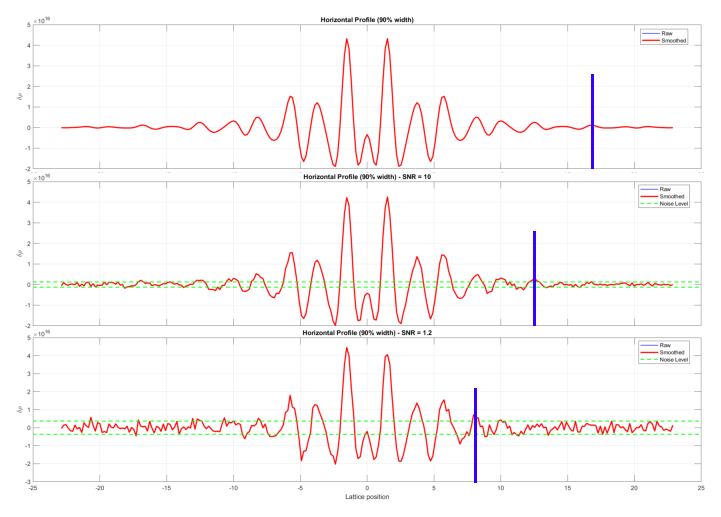
\includegraphics[width=\textwidth]{Ch5_fieldofview.pdf} 
	\centering
	\caption[\textbf{Cutoff distances of QPI patterns with different signal-to-noise ratios}]{\textbf{Cutoff distances of QPI patterns with different signal-to-noise ratios}. Three Horizontal Line profiles on $\delta\rho(\textbf{x}, E=0.45eV)$ with the noise of various levels. a) has no noise applied; b), c) have Gaussian noises applied with SNR = 10 and 1.2, respectively. Here the signal strength is defined as the variance of the noiseless $\delta\rho(\textbf{x}, E=0.45eV)$, see a) of Fig. \ref{fig:ch5_single_scattering}.}
	\label{fig:ch5_cutoff}
\end{figure}


\subsection{multi-defect QPI pattern and phase noise}
\ac{QPI} patterns present themselves around defects. While an ideal \ac{QPI} measurement is performed on isolated defects in a large field of view, it is normally difficult to find such a case. In real experiments, grid maps are usually taken on areas with multiple defects; this causes interference between the \ac{QPI} patterns originating from different defects, as hinted by Ch.4.2.3 when discussing Fig. \ref{fig:ch5_multi_scattering}.

This is problematic when we try to interpret the \textbf{q}-space \ac{QPI} map. As illustrated in Fig. \ref{fig:ch5_phasenoise}, when we have multiple defects scattered in the field of view, we start to see some noise patterns associated with the spatial distribution of the defects, as we can see by comparing c) and e), we see that with nothing but the relative locations of the defects changed, the corresponding \textbf{q}-space \ac{QPI} maps possess different noise patterns. This effect is referred to as phase noise, which hinders our ability to analyze the underlying quasiparticle scattering process. 

\begin{figure}
	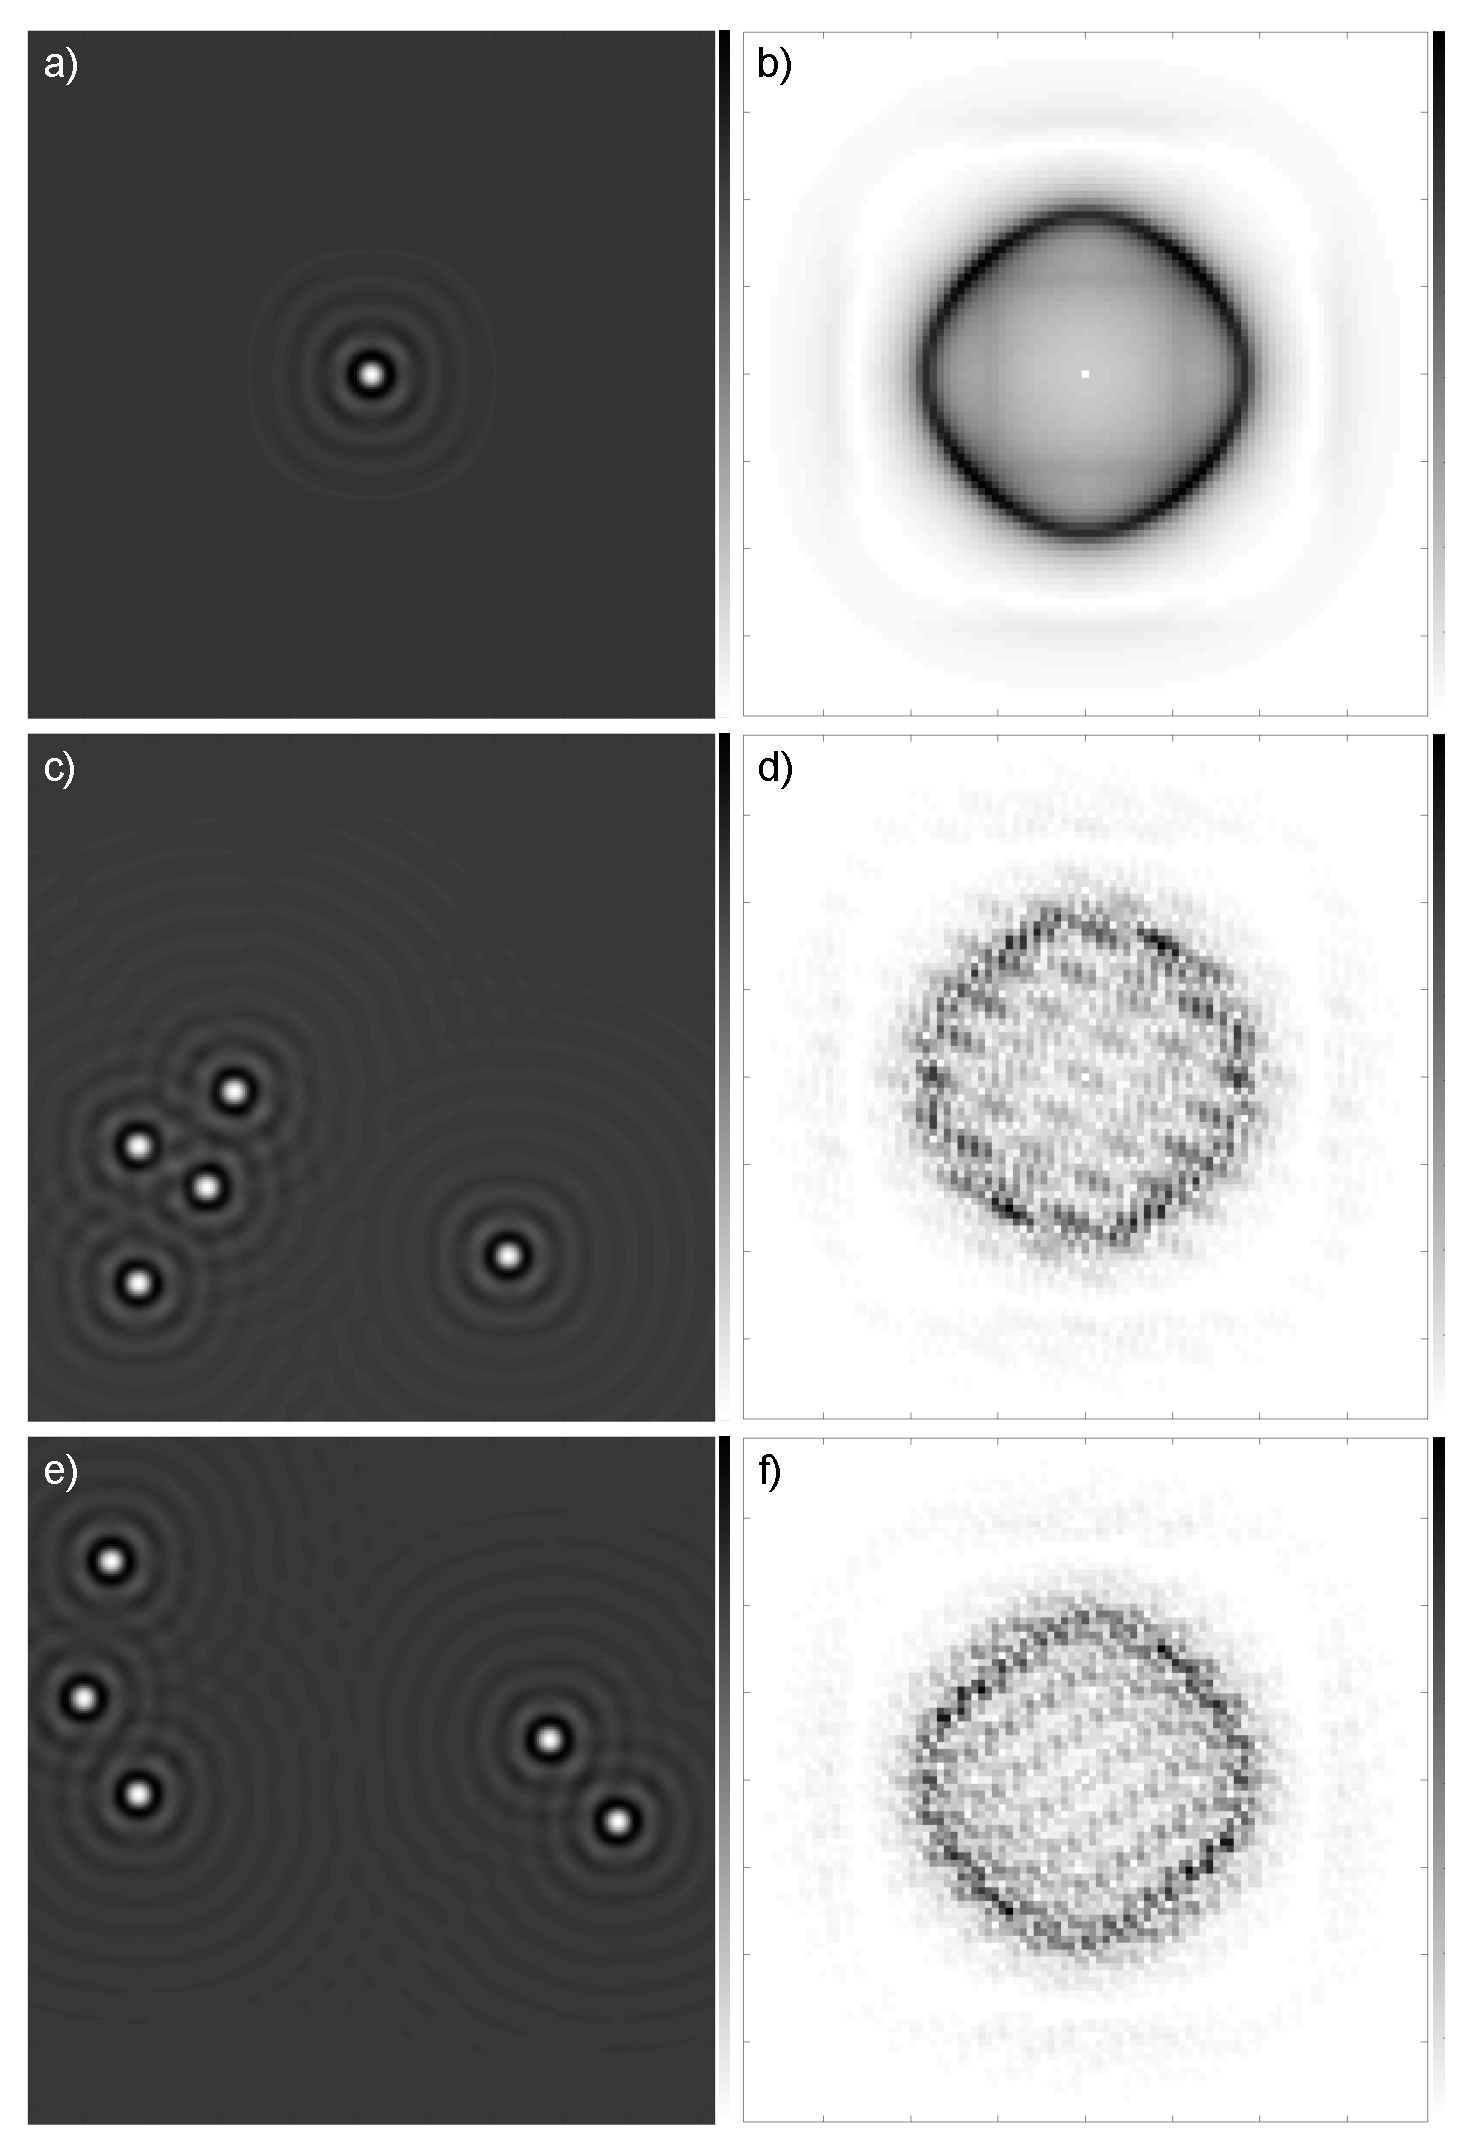
\includegraphics[width=0.85 \textwidth]{Ch5_phasenoise.pdf} 
	\centering
	\caption[\textbf{Phase noise illustration I}]{\textbf{Phase noise illustration I}. a),b): single defect scattering pattern and corresponding \textbf{q}-space QPI map. c)-f): multi-defect scattering with the same number of defects with different distributions, the corresponding QPI map presents phase noise with different patterns that associate with the defect distribution}
	\label{fig:ch5_phasenoise}
\end{figure}

Beyond the phenomenological illustration, we can further understand the source of phase noise with a mathematical analysis on multi-defect $\delta\rho(\textbf{x},\omega)$. We first discuss the form of the multi-defect T-matrix T, which is a $N_d \times N_d$ square matrix with entry T$_{\alpha \beta}$ representing the cross scattering term between defect m and n. We then separate the diagonal and off-diagonal terms and express T as \cite{leonard1972}:
\begin{align}
	\ T_{\alpha\beta} &= t_{\alpha} \delta_{\alpha\beta} + t_{\alpha} G_{0\alpha\beta} (1 - \delta_{\alpha\beta}) t_{\beta} + \sum_{\alpha' \neq \alpha, \beta} t_{\alpha} G_{0\alpha\alpha'} t_{\alpha'} G_{0\alpha'\beta} t_{\beta} + \cdots \label{eq_tmul}\\
	\label{eq.536}
	&= t_{\alpha} \delta_{\alpha\beta} + t_{\alpha} \sum_{\alpha'} \check{G}_{\alpha\alpha'} \ T_{\alpha'\beta},
\end{align}
\noindent where $t_{\alpha}$ is the T-matrix of a single impurity at site $\alpha$ and expressed on a matrix form in a localized basis set (i.e., expressed as the matrix with the same dimension as the multi-defect case but with only the $\alpha$'s diagonal entry none empty). And matrix $\check{G}_{\alpha\alpha'} = G_{0\alpha\alpha'}(1-\delta_{\alpha\alpha'})$, it contains the off-diagonal part of the Green's function. It has been shown by Fang et al. \cite{fangTheoryQuasiparticleInterference2013} that, in the Born approximation to the scattering amplitude, the first term dominates over the second term, and the latter can be omitted. We can, therefore, approximate multi-defect scattering with multiple single-defect scattering events. 

This approximation was then extended to the strong scattering case by Philipp et al. \cite{russmannInitioTheoryFourierTransformed2021}, under the assumption that the impurity concentration is low and the largest part of the surface is covered by pristine atoms and far from the impurities. They then utilized Equation \ref{eq.536} and further expressed the Green's function difference:

\[
\Delta G(\mathbf{r}, \mathbf{r}, E) = \int d^3 \mathbf{r}' \int d^3 \mathbf{r}'' \, G_0(\mathbf{r}, \mathbf{r}'; E) \, T(\mathbf{r}', \mathbf{r}''; E) \, G_0(\mathbf{r}'', \mathbf{r}; E)
\]

\begin{align}
	\label{eq.537}
	\Delta G_{\alpha \alpha} &= \Delta G^{(1)}_{\alpha \alpha} + \Delta G^{(2)}_{\alpha \alpha} \\
	\label{eq.538}
	&= \sum_{\alpha'} G_{0\alpha \alpha'} t G_{0\alpha' \alpha} + \sum_{\alpha'} G_{0\alpha \alpha'} t\sum_{\beta \beta'} \check{G}_{\alpha' \beta} \, T_{\beta \beta'} G_{0\beta' \alpha}.
\end{align}

\noindent By applying the stationary phase approximation \cite{lounisTheoryRealSpace2011} to $G_{0\beta'\alpha}$, and utilize the translational symmetry of Bare lattice Green's function $G_0$, they showed:
\begin{equation}
	\label{eq.539}
	\Delta G^{(2)}_{\alpha\alpha}=\sum_{\alpha'}G_{0\alpha\alpha'}t\sum_{\beta\beta'}\check{G}_{\alpha'\beta}T_{\beta\beta'}K_{\beta'\alpha}e^{ik_{\beta'\alpha}\cdot R_{\beta'\alpha}},
\end{equation}

\noindent where $R_{\beta'\alpha}$ indicates the real-space displacement between defect $\beta'$ and $\alpha$. In the Fourier transform, the contribution from the phase $e^{ik_{\beta'\alpha}\cdot R_{\beta'\alpha}}$ can not be lifted, and is the source of the phase noise we observed in Fig. \ref{fig:ch5_phasenoise}. However, the contribution of the phase can be practically canceled if we sum over all configurations of randomly distributed defects, which correspond to an infinitely large scanning surface that can never be achieved. Nevertheless, a decreased influence of this phase noise can be seen if we increase the density of the defects, as illustrated in Fig \ref{fig:ch5_changephasenoise}. This is because the patterns created by the phase noise become more fine-grained and can eventually be seen as featureless, similar to the random distribution of noise.  


%todo: verify whether this is true with more literature reviews. 

\subsubsection{Phases in QPI}
As discussed in the last section, our ability to probe the quasiparticle band structure is hindered by the pattern in \textbf{q}-space from the multi-defect interference effect. Thus, we portray this pattern as the phase noise. However, we should clarify that this multi-defect phase effect contains information about the relative spatial distribution of the defects and, thus, is not strictly noise. A more accurate name for this effect is speckles. In laser physics, when an optically rough object is illuminated with coherent laser light, and the diffusely backscattered light is collected on a screen, the backscattered light will create an interference pattern on this screen, and this interference pattern is referred to as the speckles\cite{ReviewLaserSpeckle}.

There are also many sources of phase changes in \ac{STM} and \ac{QPI} measurement; more specifically, phase changes can be introduced in 3 ways: 
\begin{itemize}
	\item Different defect potentials can introduce different phase changes during the scattering process; this may select certain channels of scatterings and produces different QPI patterns around different defects. \cite{chenAtomicallyResolvedDefectEngineering2024}
	\item Different spatial distributions of the defects, as we discussed extensively above. 
	\item When performing FFT power spectrum, a phase term is eliminated, making the \textbf{q}-space \ac{QPI} invariant under real-space translations.
\end{itemize}

Therefore, the name speckle is not only more accurate in describing the effect but also more precise in distinguishing it from phase effects from other sources. Thus, we will abandon the colloquial term "Phase noise" and use "Speckle" to describe this multi-defect interference effect. 

Now, with the proper setup of this challenge to resolve quasiparticle band structure with speckles, we will introduce a method that addresses it. 

\begin{figure}
	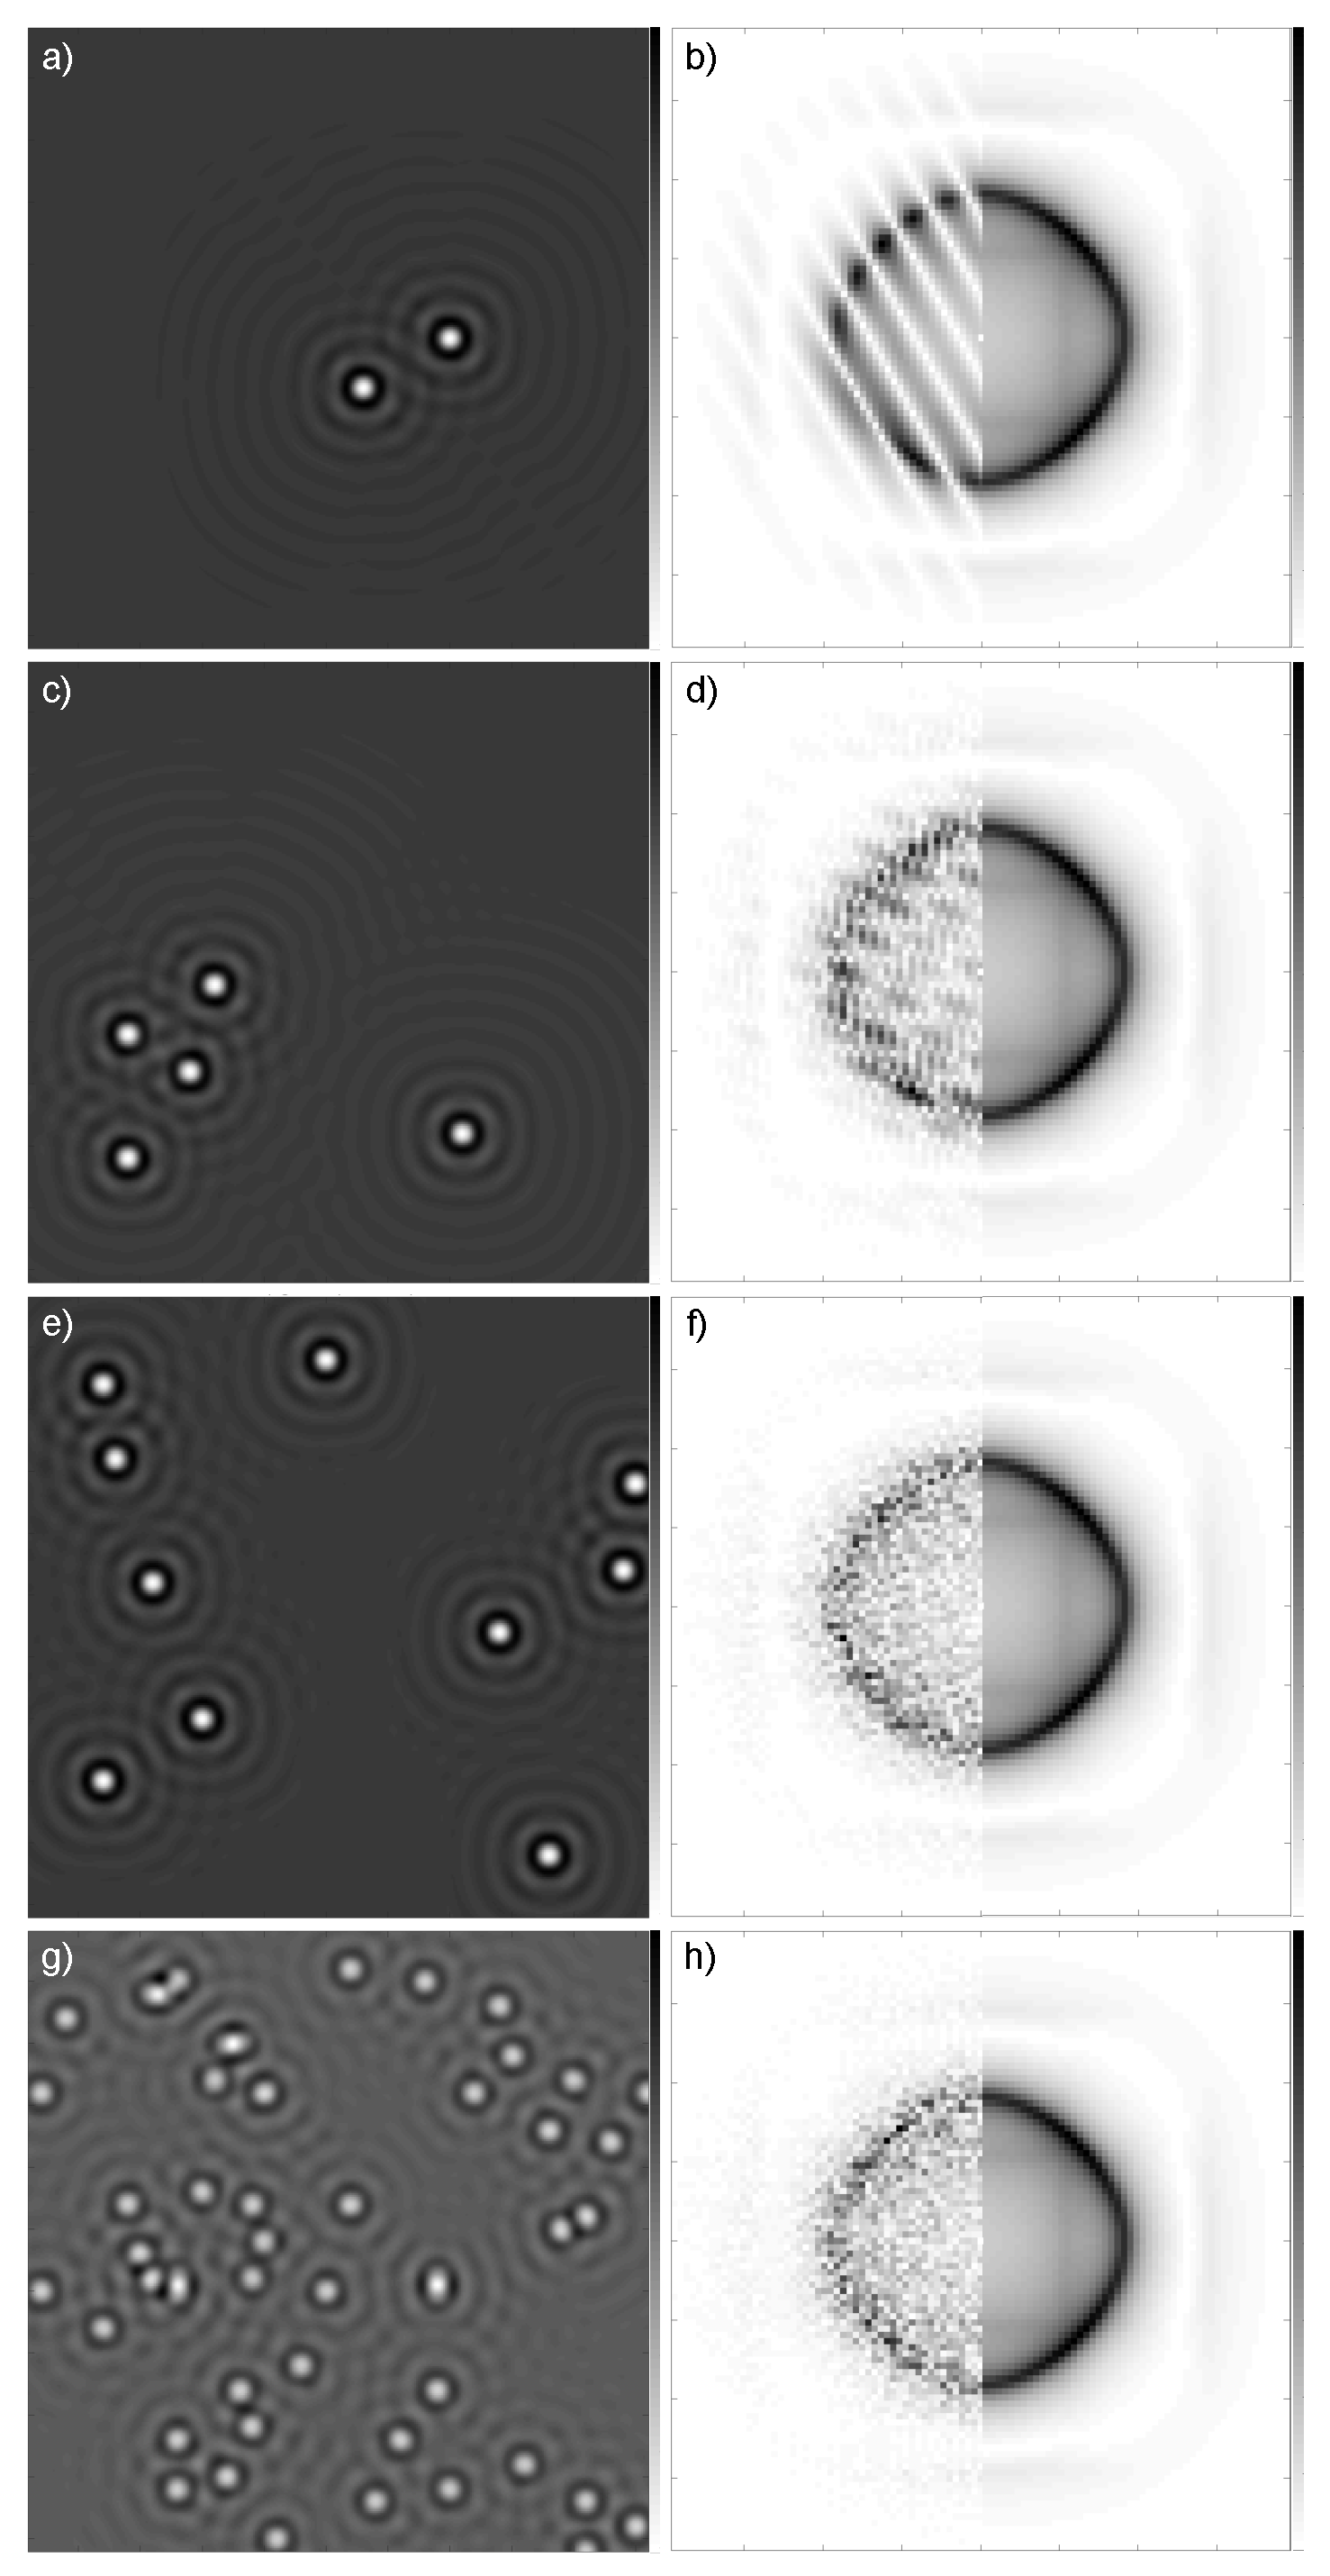
\includegraphics[width=0.7 \textwidth]{Ch5_changephasenoise.pdf} 
	\centering
	\caption[\textbf{Phase noise illustration II}]{\textbf{Phase noise illustration II}. The effect of the phase noise is most prominent in the sparse defects regime. a)-h): $\delta\rho(\textbf{r},\omega)$ and \textbf{q}-space QPI plotted in pair with increasing defect concentration, showing the phase noise becomes more featureless. Single-defect QPI map is presented for reference on the right half of the \textbf{q}-space QPI.}
	\label{fig:ch5_changephasenoise}
\end{figure}
